\graphicspath{
    {figures_and_references/urban_surface_detection/}
    {figures_and_references/footprints_paper/}
    {figures_and_references/EELISA_conference/}
}

% \selectlanguage{english}
\renewcommand{\chapternametext}{Chapter \thechapter: Footprint-derived seismic exposure attributes}

\begin{refsection}

\chapter{\chapternametext}
\

\renewcommand{\headingtextL}{}
\renewcommand{\headingtextR}{\chapternametext}
\begingroup
 \flushbottom
 \setlength{\parskip}{0pt plus 1fil}%
 \localtableofcontents 
\endgroup

\begingroup
 \flushbottom
 \setlength{\parskip}{0pt plus 1fil}%
 \locallistoffigures
 \locallistoftables
\endgroup


\newpage

\setcounter{section}{0} 



\FloatBarrier

\renewcommand{\sectionnametext}{Structural simplifications and assumptions}
\renewcommand{\headingtextL}{\chapternametext}
\renewcommand{\headingtextR}{\thesection. \sectionnametext}
\section{\sectionnametext}
\label{sec:simplifications}

\begin{figure}[htbp]
    \centering
    \includegraphics[width=0.6\linewidth]{figures/box_idealization_and_eccentricity.jpg}
    \caption{Idealization of a building as a rigid box.}
    \label{fig:idealization}
\end{figure}

Building codes typically define structural irregularity based on detailed design considerations, such as material properties and the configuration of load-resisting elements. In contrast, the present methodology is restricted to footprint geometry and plan-based configuration, deliberately excluding structural materials, internal resisting systems, and other building-level characteristics that cannot be reliably inferred from geospatial data alone. For this reason, the proposed workflow should be understood as a first-order approximation of seismic behaviour modifiers derived from building footprints. To ensure transparency, the assumptions and limitations underlying this approximation are stated explicitly below.

First, all openings such as windows and doors are ignored. Walls are assumed to be continuous, of uniform thickness and composed of identical materials. Second, every wall is considered a structural element. It is also assumed that the building consists of one storey per three metres in height. For simplification, only a single storey is modelled, with floor and ceiling slabs of the same thickness and material properties as the walls. In this representation, the building is conceptualized as a hollow box, with structural resistance provided entirely by the walls.

An additional assumption is that each footprint corresponds to a single structural unit. Consequently, the methodology cannot directly identify cases in which a large apparent footprint is actually composed of two or more structurally independent bodies separated by expansion or seismic joints. In such situations, the full footprint may be analysed as a single building, which may lead to an overestimation of plan irregularity or to the assignment of an inappropriate behaviour modifier. Likewise, internal structural subdivisions or discontinuities that are not expressed in the external footprint cannot be captured by the proposed approach. Accordingly, the modifiers derived in this study must be interpreted with this constraint in mind, since the position within the block, the assessment of plan irregularity, and the classification of footprint shape are all established from the apparent external footprint and may therefore differ from the actual structural configuration when multiple independent units are aggregated within a single mapped outline or when structural joints are not externally discernible.

As a result of these assumptions (fig. \ref{fig:idealization}), the analysis is limited to code-based metrics that depend on geometric attributes observable in plan. The methodology is therefore intended to improve large-scale exposure assessment in data-scarce environments, rather than to replace detailed structural surveys or building-specific engineering assessment.



\subsection{Centre of mass and centre of stiffness}

The centre of mass ($\mathbf{r}_{\text{cm}}$) as the weighted average of the centroids of two surfaces: the ceiling and the walls (eq \ref{eq:centroid_avg}). The centroid of the ceiling corresponds to the centroid of the footprint polygon, while the centroid of the walls corresponds to the centroid of the boundary geometry of the footprint. The weights used in this averaging are the footprint area ($A$) for the ceiling and the product of the boundary length ($\ell$) and the assumed wall height (3 metres) for the walls. The $z$ coordinate of the centre of mass is neglected as in this study only 2D footprints are considered.

\begin{equation}
    \label{eq:centroid_avg}
    \mathbf{r}_{\text{cm x,y}} = \frac{\operatorname{centroid}(\text{footprint}) \cdot A + \operatorname{centroid}(\text{boundary}) \cdot \ell \cdot 3}{A + \ell \cdot 3}
\end{equation} 

If additional floors are considered, the centre of mass remains unchanged, since each floor includes a ceiling and 3-meter-high walls with consistent characteristics.

The centre of stiffness corresponds to the centre of mass of the lateral-force-resisting elements, the walls. Thus, it is defined as the centroid of the footprint boundary geometry.

\subsection{Basic footprint lengths}

To evaluate footprint shape and irregularity, seismic codes typically reference idealized building shapes (e.g., squares, L-shapes, and T-shapes) with standardized side lengths. For arbitrary footprints, determining relevant dimensions requires a generalized approach. Two principal methods are used for this purpose: the second moment of area and the minimum bounding box.

\begin{enumerate}
    \item \textbf{Second Moment of Area}

    The second moment of area is calculated as $I_x = \int y^2\,dA$, where $x$ and $y$ are arbitrary perpendicular axes and $dA$ is an infinitesimal area element. In all equations, $I_1$ and $I_2$ represent the largest and smallest principal moments, respectively, for the footprint polygon.

    \begin{itemize}
        \item \textbf{Slenderness}: For a rectangle with sides $a > b$, slenderness is defined as $\frac{a}{b}$. This ratio can be related to the ratio of principal moments $\frac{I_1}{I_2}$. Using dimensional analysis, since both $I_1$ and $I_2$ are in units of $[m^4]$, the slenderness is approximated as:

        \begin{equation}
            \label{eq:slenderness_I}
            \text{Slenderness} = \sqrt{\frac{I_1}{I_2}}
        \end{equation}

        For a rectangular footprint, this yields:
        \[
        \sqrt{\frac{\frac{1}{12}ba^3}{\frac{1}{12}ab^3}} = \sqrt{\frac{a^2}{b^2}} = \frac{a}{b}
        \]

        \item \textbf{Side Length}: The side length in the direction perpendicular to the axis of the largest principal moment ($I_1$) is computed as:

        \begin{equation}
            \label{eq:side_I}
            \text{Side Length} = \sqrt{\text{Area} \times \text{Slenderness}}
        \end{equation}

        The side length in the direction perpendicular to the smallest moment ($I_2$) is then computed by dividing the area by the length calculated above.

        For example, with a rectangle of area $A = ab$ and slenderness $\frac{a}{b}$, we get:
        \[
        \sqrt{ab \cdot \frac{a}{b}} = \sqrt{a^2} = a
        \]

        This method yields an average side length in each principal direction (fig \ref{fig:L_SMA}).

    \end{itemize}

    \item \textbf{Minimum Bounding Box (MBB)}

    A rectangle can be circumscribed around the footprint similarly to how a circle is inscribed. Multiple such rectangles are possible, and the \emph{minimum bounding box} (MBB) is the one with the smallest area \footcite{chaudhuri_simple_2007} (fig \ref{fig:L_MBB}).

    \begin{itemize}
        \item \textbf{Slenderness}: The slenderness of the footprint is defined by the aspect ratio of the MBB. This approach typically results in lower slenderness values compared to the second moment of area method (fig \ref{fig:side_length}).

        \item \textbf{Side Length}: The side lengths are simply the side dimensions of the MBB (fig \ref{fig:L_MBB}).
    \end{itemize}
\end{enumerate}

\begin{figure}[htbp]
    \centering
    \begin{tabular}{cc}
        \begin{subfigure}[t]{0.45\linewidth}
            \centering
            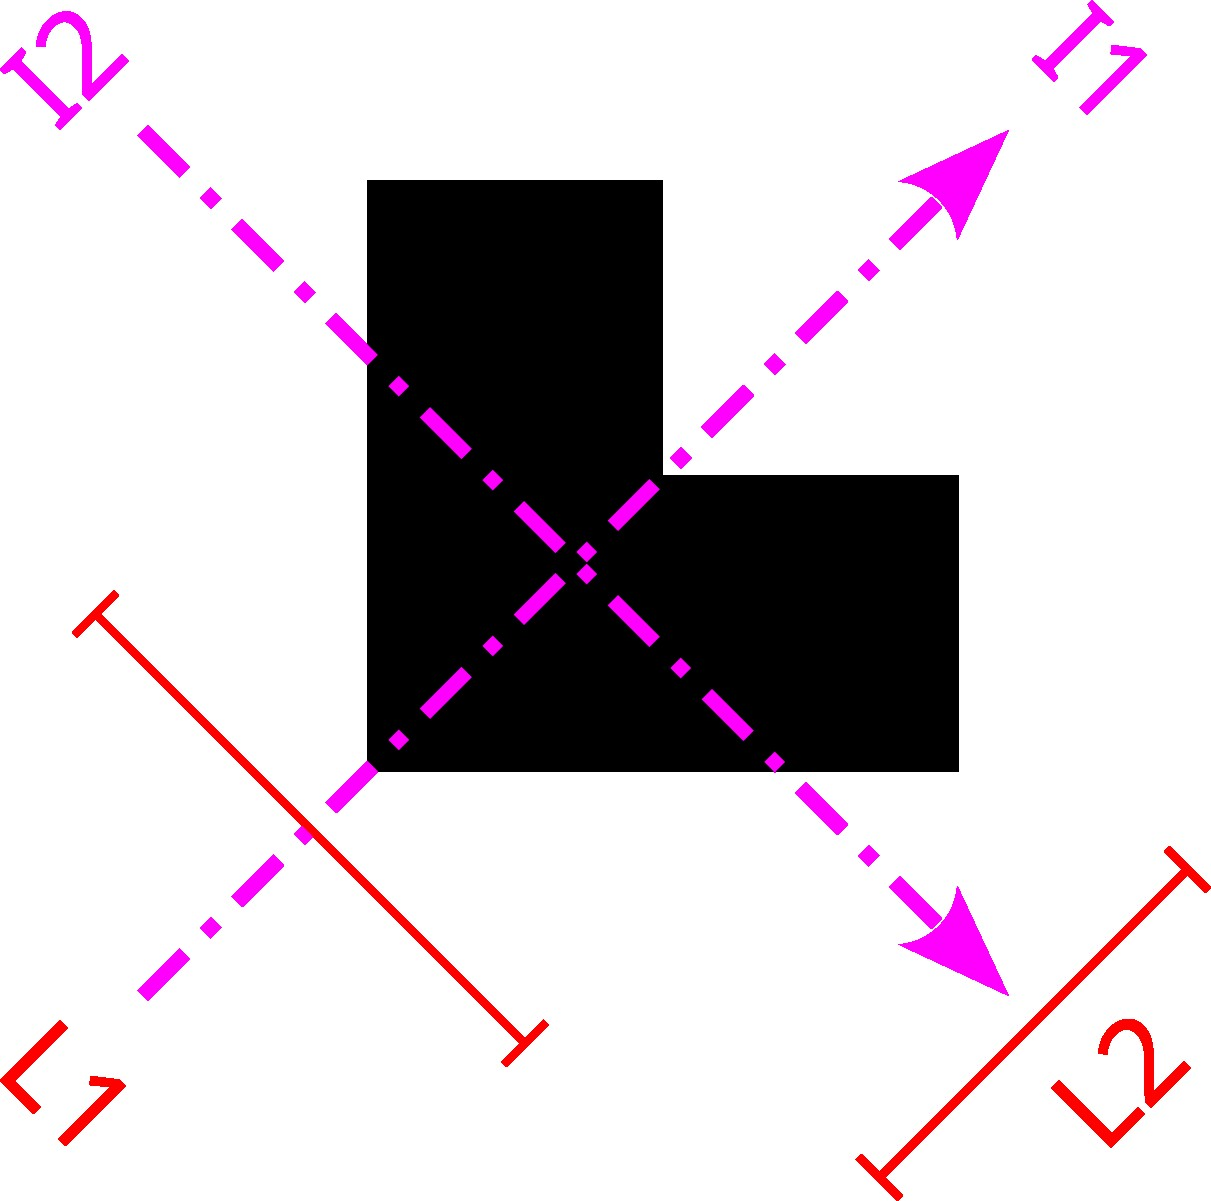
\includegraphics[width=0.85\linewidth]{figures/axis_inertia_2b.jpg}
            \caption{L-shaped footprint with axes aligned to principal directions (second moment of area).}
            \label{fig:L_SMA}
        \end{subfigure} &
        \begin{subfigure}[t]{0.45\linewidth}
            \centering
            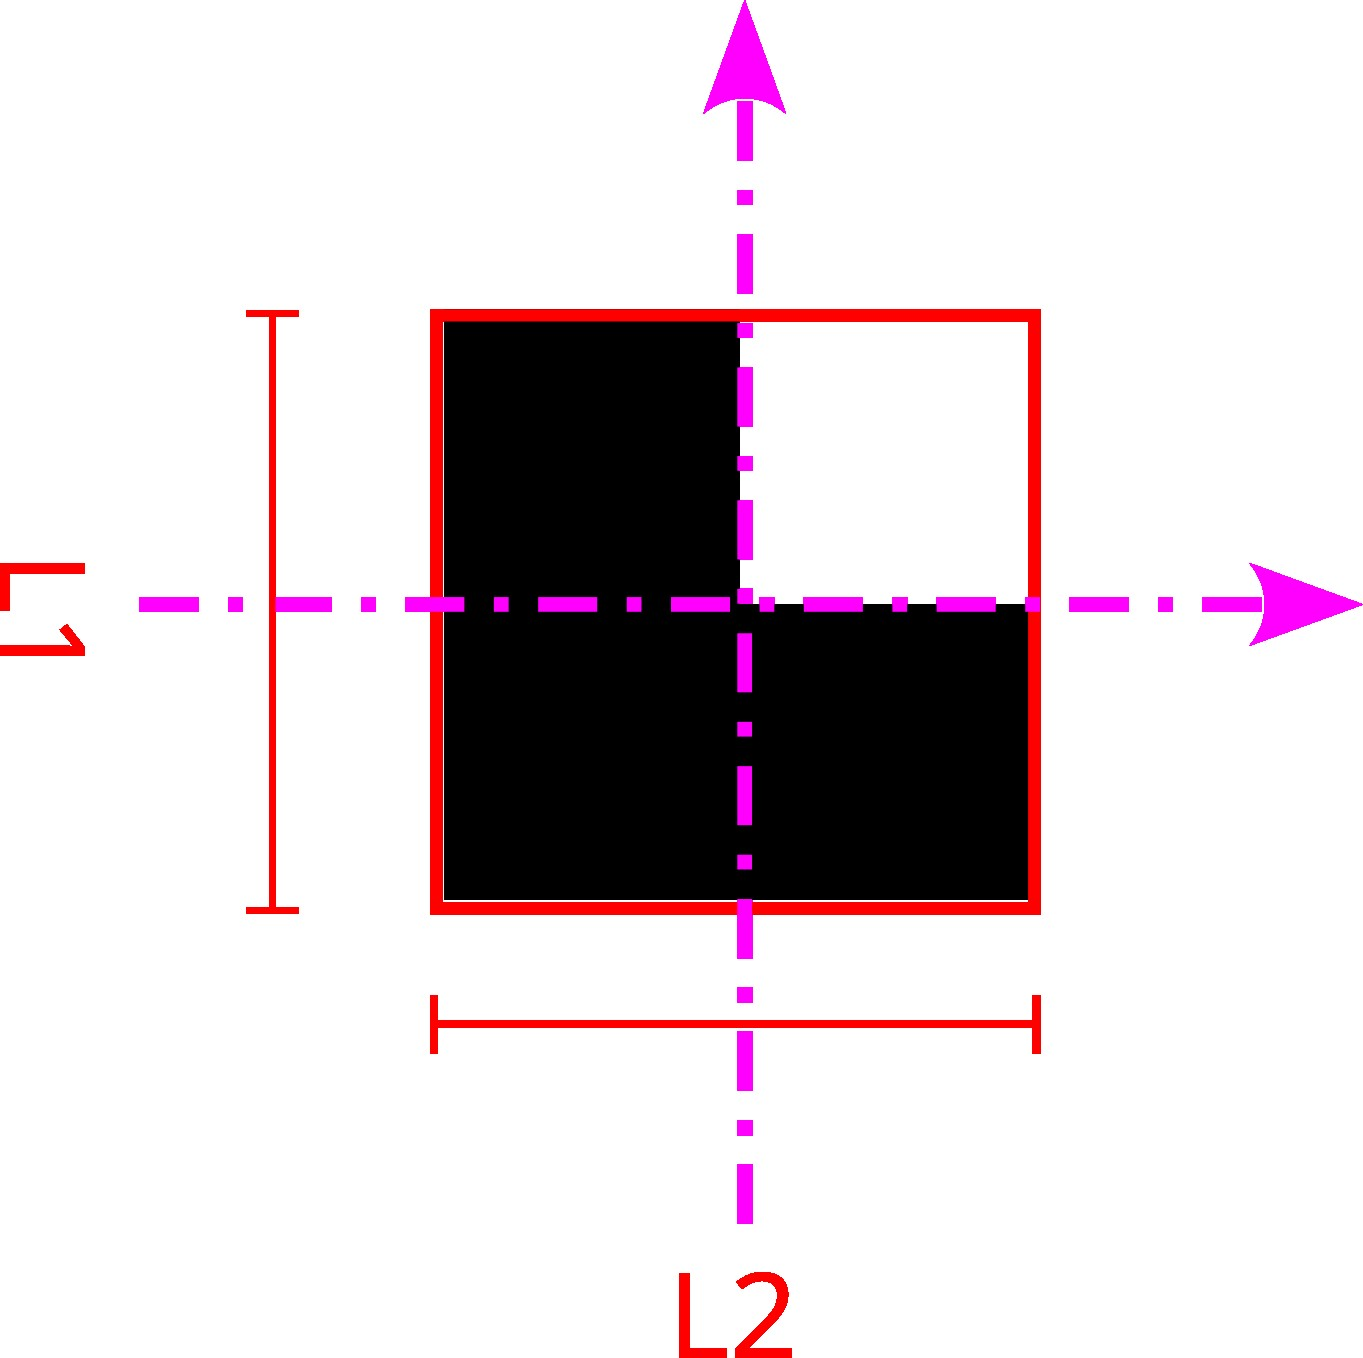
\includegraphics[width=\linewidth]{figures/axis_inertia_3.jpg}
            \caption{L-shaped footprint with axes aligned to minimum bounding box.}
            \label{fig:L_MBB}
        \end{subfigure}
    \end{tabular}
    \caption{Comparison of side lengths derived using the second moment of area and minimum bounding box methods.}
    \label{fig:side_length}
\end{figure}


\renewcommand{\sectionnametext}{Building position within the block}
\renewcommand{\headingtextR}{\thesection. \sectionnametext}
\section{\sectionnametext}

To determine the position of the building within the block, a methodology was designed based on the simulation of contact forces in all sides of the building footprint polygons and the analysis of resultant forces. For this purpose, contact forces on all contact surfaces are calculated by applying a virtual unit pressure $1\text{ Pa}$ to each contact surface and calculating the resultant force, which is then placed in the centre of each contact surface (fig \ref{fig:rel_pos_exp}). When the height of the building is unknown, all buildings are assumed to have a height of 1 metre. If the height is known, the contact force is divided by the height of the building to normalise the values. The contact force serves as an analogy to produce normalized, direction-aware contact metrics.
While the terminology used (force, momentum, acceleration) is mechanical, these parameters function here as direction-aware geometric proxies. Unlike simple shared-boundary lengths, these metrics allow the algorithm to distinguish between symmetric confinement and asymmetric contact that may induce torsional responses.


A buffer is applied to the building footprint based on the minimum detectable distance, which depends on the resolution of both the digital footprint data and the underlying aerial imagery. This is a critical step, as it helps avoid underestimating or overestimating building contacts. Nevertheless, very small separations that technically isolate buildings ($> 5cm$) may remain undetectable. Therefore, the relative position of buildings should only be considered when it has a detrimental effect on their seismic response. 


\begin{figure}[htbp]
    \centering
    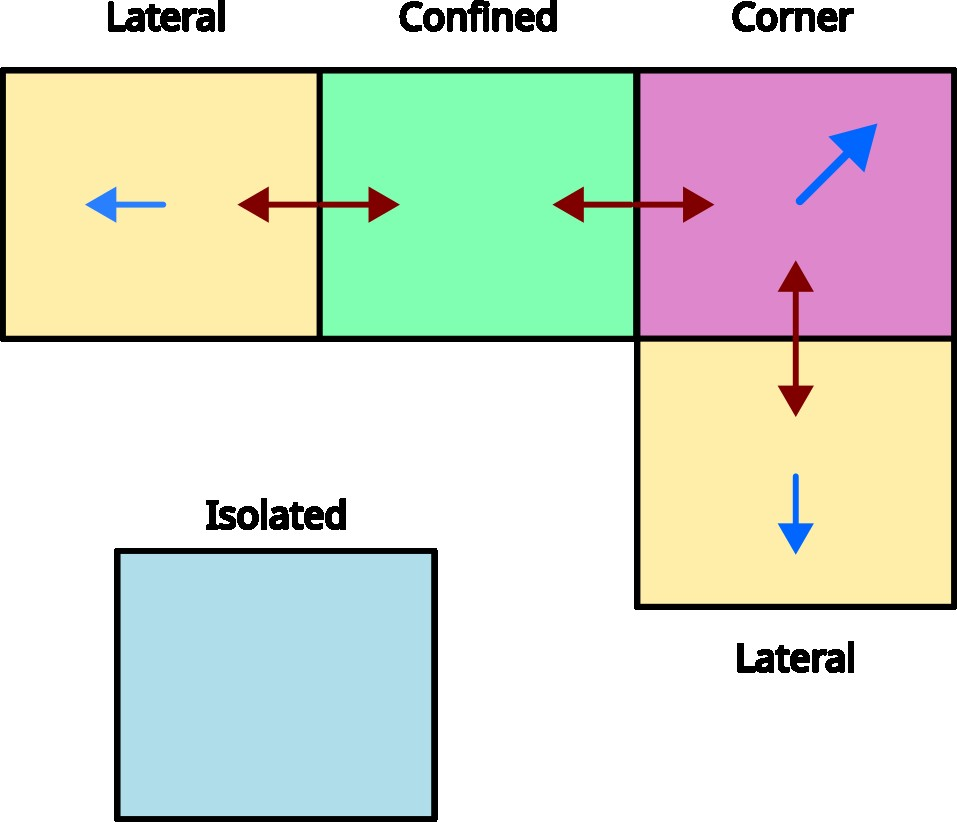
\includegraphics[width=0.4\linewidth]{figures/relative_position_explanation.jpg}
    \caption{Relative positions and contact points are important: red arrows represent individual contact forces, while the blue arrow shows the resultant contact force.}
    \label{fig:rel_pos_exp}
\end{figure}

Considering all contact forces acting on the footprint, four indices can be computed:

\begin{itemize}
\item \textit{angular\_acc}: The angular acceleration is computed following equation \ref{eq:ang_acc} (with $F_i$ contact force $i$, $A$ area of the footprint, $I_z$ second moment of area and $M$ momentum).

\begin{equation}
    \label{eq:ang_acc}
    \text{angular acc} = \frac{M \cdot A}{I_z}
\end{equation} 

  Where \textit{momentum} $(M)$ is computed following equation \ref{eq:mom} (with $d_i$ being the distance to the centre of mass):

\begin{equation}
    \label{eq:mom}
    M = \sum_{i} d_i \cdot F_i
\end{equation} 

\item \textit{force}: The magnitude of the resultant contact force acting on the footprint, normalised by the square root of the area of the footprint (eq \ref{eq:force}).

\begin{equation}
    \label{eq:force}
    \text{force} = \frac{\left| \sum_{i} F_i \right|}{\sqrt{A}}
\end{equation} 

\item \textit{confinement\_ratio}: The confinement ratio represents the proportion of total contact forces that are confined or counterbalanced as the ratio of the confined force divided by the sum of the absolute value of all forces. The confined force is calculated by subtracting the squared sum of the magnitudes of all contact forces ($\sqrt{\sum_{i} |F_i|^2}$) the magnitude of the resultant force ($\left| \sum_{i} F_i \right|$). The range of this parameter would be 0 (no confinement)-1 (total confinement).
    \begin{equation}
        \label{eq:conf}
        \text{confinement\_ratio} = \frac{\sqrt{\sum_{i} \left| F_i \right|^2} - \left| \sum_{i} F_i \right|}{\sqrt{\sum_{i} \left| F_i^2 \right|} }
    \end{equation}

\item \textit{weighted\_angle}: The sum of the angles between individual contact forces, weighted by the magnitude of the contact force (eq \ref{eq:angle}).

\begin{equation}
    \label{eq:angle}
    \text{weighted\_angle} = \frac{\sum_{i}\left[ \left|F_i\right| \cdot \angle(F_i, \sum_{j} F_j)\right]}{\sum_{i}\left|F_i\right|}
\end{equation} 

\end{itemize}

Relative position classes are defined as follows:

\begin{enumerate}
    \item \textbf{“torque”}: Opposing forces could produce torque on the building. High \textit{angular acceleration} and criteria for classes \textit{confined} or \textit{corner} are met.
    \item \textbf{“confined”}: Touches on both lateral sides. The \textit{confinement ratio} is high.
    \item \textbf{“corner”}: Touches on two perpendicular sides. The \textit{angle} is high and the criteria for \textit{lateral} are met.
    \item \textbf{“lateral”}: Touches on one side. The \textit{force} is high.
    \item \textbf{“isolated”}: No touching structures. None of the above criteria are met.
\end{enumerate}

The threshold for considering a value as "high" can vary and should be defined by the user. However, the \texttt{SeismicBuildingExposure} package includes default values established by experts based on idealized cases. These default thresholds are set to:

\begin{itemize}
    \item \textit{angular acceleration} $> 2.133$: Would be the result of touching structures covering $1/3$ of two opposing sides of a building footprint with a rectangular shape and slenderness $2$. Contact forces would be positioned producing the maximum possible amount of torque. 
    \item \textit{force} $> 0.1666$: Would be the result of a touching structure covering $1/6$ of the side of a square building footprint.
    \item \textit{confinement ratio} $> 0.5$: If there are more confined forces than non-confined forces the confinement ratio is considered high.
    \item \textit{angle} $> 0.78$: Would be $\pi / 4$ radians or $45$ degrees. 
\end{itemize}

Experts assigned visually relative position classes to the building footprints in the three pilot regions for evaluation.


\vspace{1em} 

\renewcommand{\sectionnametext}{Direction}
\renewcommand{\headingtextR}{\thesection. \sectionnametext}
\section{\sectionnametext}


The building direction is defined as the direction of the principal axis associated with the maximum second moment of area of the footprint geometry. This direction is computed as the angle between grid north in the adopted UTM coordinate system and the eigenvector associated with the minimum principal direction. This axis is adopted because it is associated with the smallest transverse resisting dimension and is therefore considered the most unfavorable direction with respect to seismic action.

\renewcommand{\sectionnametext}{UNE-EN 1998-1 Eurocode 8 (2004)}
\renewcommand{\headingtextR}{\thesection. \sectionnametext}
\section{\sectionnametext}
\label{sec:EC8}

Eurocode 8 (EC8) \footcite{en_1998_en1998_2011} provides the primary framework for assessing seismic actions and structural response in buildings within European standards. Within this framework, certain dynamic response parameters are essential for evaluating structural irregularities. Some of these parameters, such as eccentricity and torsional radius, are not purely geometric in nature. However, under the assumptions outlined in section \ref{sec:simplifications} and following the provisions of EC8, they can be computed as follows:


\begin{itemize}
\item \textbf{Eccentricity} ($e$): Distance between the centre of mass and the centre of stiffness. 

\item \textbf{Torsional radius} ($r_t$): Calculated following equation \ref{eq:r_t}, where $I_t$ is the second moment of area of the footprint polygon in the Z-direction through the centre of stiffness and $I_j$ is the second moment of area of the footprint polygon through the centre of mass along the axis perpendicular to the calculation direction in the plain of the polygon.
\begin{equation}
    \label{eq:r_t}
    r_t = \sqrt{\frac{I_t}{I_j}}
\end{equation}

\item \textbf{Radius of gyration} ($r_g$): Calculated following equation \ref{eq:r_g}, where $I_0$ is the second moment of area of the footprint polygon in the Z-direction through the centre of mass.
\begin{equation}
    \label{eq:r_g}
    r_g = \sqrt{\frac{I_0}{\text{area}}}
\end{equation}.

\end{itemize}

The Eurocode 8 parameters that were implemented into the \textit{SeismicBuildingExposure} package are: 

\begin{itemize}
    \item \textbf{Eccentricity ratio}: Worst possible value in any direction in the footprint plain outputted by equation \ref{eq:ecc_ratio_EC}.
    \begin{equation}
        \label{eq:ecc_ratio_EC}
        \text{eccentricity\_ratio} = \frac{e}{r_t}
    \end{equation}


    This parameter measures general irregularities in the resisting element, the wall or footprint boundary. In the Eurocode it is limited to $0.3$ %\textbf{REVISAR Y QUIZAS AÑADIR FIGURA}.
    
    \item \textbf{Radius ratio}: Calculated according to equation \ref{eq:radius_ratio}. 
    \begin{equation}
        \label{eq:radius_ratio}
        \text{radius\_ratio} = \frac{r_t}{r_g}
    \end{equation}

    This parameter is limited in the Eurocode 8 (Ec8) to $1$. Both eccentricity ratio and radius ratio are part of the same parameter and both limits should be met.  

    
    \item \textbf{Slenderness}: Computed following the second moment of inertia or the bounding-box approach.


    Slenderness is related to a direction in which the building is weaker as less elements resist lateral forces in the thinnest direction. The SeismicBuidlingExposure library can output the angle of the weak direction (towards the north in UTM coordinates). By default the recommended method of the second moment of area is used but the minimum bounding box is an available alternative. The Ec8 limits this parameter at 4.

    
    \item \textbf{Compactness}: The compactness is calculated by first computing the set difference between the footprint without holes (fig \ref{fig:compactness_1}) and its convex hull (fig \ref{fig:compactness_1}). The total area of the resulting polygons is measured, and compactness is defined as one minus the ratio of the largest resulting polygon's area to the original footprint area.
    
    
    %This parameter is defined as one minus the ratio of the area of the difference of the convex hull (fig \ref{fig:compactness_2}) and the footprint and the area of the footprint (without holes) \ref{fig:compactness_1}). 

    \begin{figure}[htbp]
        \centering
        \begin{tabular}{cc}
            \begin{subfigure}[t]{0.45\linewidth}
                \centering
                
\includegraphics[width=0.5\linewidth]{figures/compactness_1.jpg}
                \caption{Footprint geometry (black) and convex hull boundary (green).}
                \label{fig:compactness_1}
            \end{subfigure} & 
            \begin{subfigure}[t]{0.45\linewidth}
                \centering
                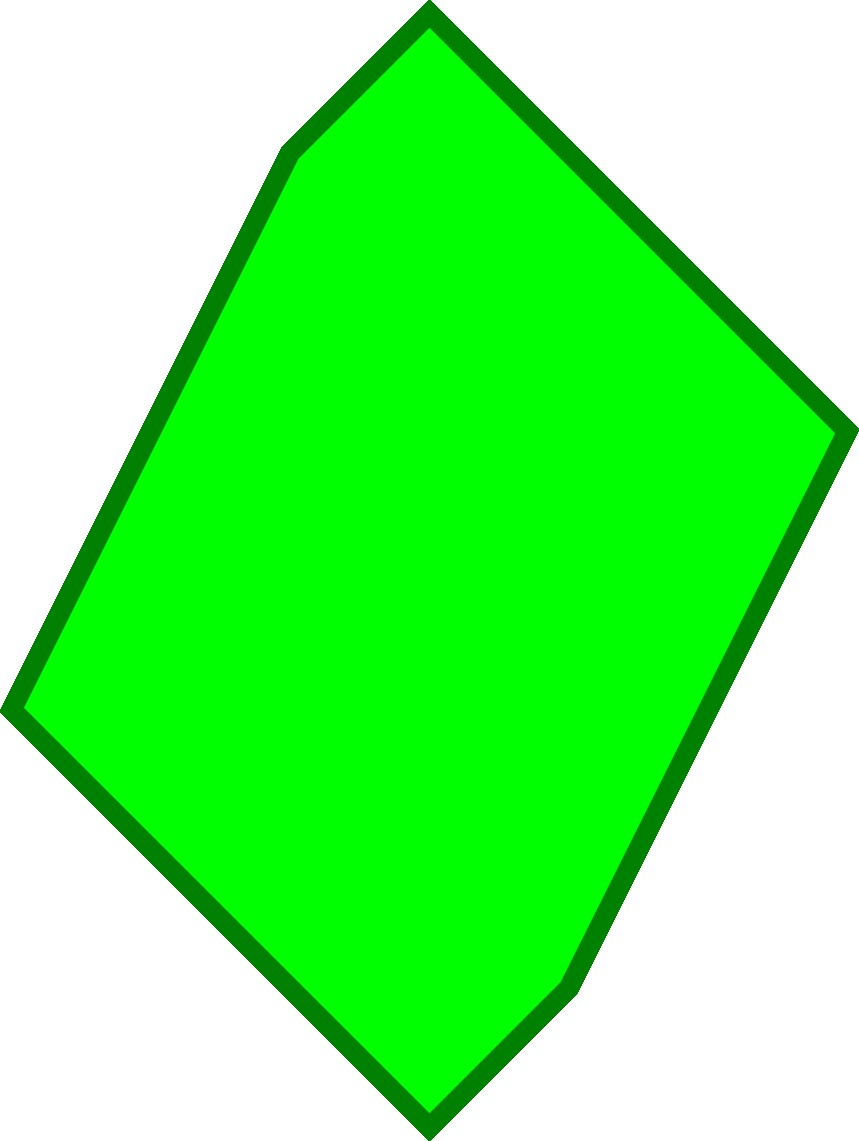
\includegraphics[width=0.5\linewidth]{figures/compactness_2.jpg}
                \caption{Convex hull geometry.}
                \label{fig:compactness_2}
            \end{subfigure}
        \end{tabular}
        \caption{Convex hull of a footprint geometry.}
        \label{fig:compactness}
    \end{figure}

    Shapes that are not compact have parts that concentrate tensions in some surfaces. This parameter measures the general amount or the total area of setbacks in the footprint. The Ec8 limits this parameter at 0.95. 
\end{itemize}

The limits set by Ec8 are summarised in table \ref{tab:EC8_limits}. 

\begin{table}[h]
    \centering
    \caption{Limitations of each irregularity parameter according to the Eurocode 8.}
    \begin{tabular}{|c|c|}
        \hline
        \textbf{Parameter} & \textbf{Limit}\\
        \hline
        \textbf{Eccentricity ratio} & $\leq 0.3$\\
        \hline
        \textbf{Radius ratio}  & $\leq1$\\
        \hline
        \textbf{Slenderness}  & $\leq4$\\
        \hline
        \textbf{Compactness}  & $\ge0.95$\\
        \hline
    \end{tabular}
    \label{tab:EC8_limits}
\end{table}


\FloatBarrier

\renewcommand{\sectionnametext}{CSCR 2010. Costa Rica Seismic Code}
\renewcommand{\headingtextR}{\thesection. \sectionnametext}
\section{\sectionnametext}
\label{sec:CSCR}

The Costa Rica Seismic Code (CSCR2010) \footcite{cfia_colegio_federado_de_ingenieros_y_arquitectos_de_costa_rica_codigo_2016} limits footprint irregularity with a parameter similar to the eccentricity ratio in the Eurocode. 

\begin{itemize}
    \item \textbf{Eccentricity ratio}: Calculated according to equation \ref{eq:ecc_ratio_CR}, where $l$ is the side length of the building calculated after the second moment of the area or the minimum bounding box approach. 
    \begin{equation}
        \label{eq:ecc_ratio_CR}
        \text{eccentricity ratio} = \frac{e}{l}
    \end{equation}
    The side length is not parallel to the principal directions. It is the one in the direction that produces the maximum eccentricity ratio. 
\end{itemize}

The eccentricity ratio is limited in the code to the values given in table \ref{tab:CR_limits}. 

\begin{table}[h]
    \centering
    \caption{Limitations of the Costa Rica Seismic Code for the eccentricity ratio.}
    \begin{tabular}{|c|c|c|}
        \hline
        \textbf{Parameter} & \textbf{Limit} & \textbf{Irregularity Level}\\
        \hline
        \textbf{Eccentricity ratio} & $\leq 0.05$ & Regular\\
        \hline
        \textbf{Eccentricity ratio}  & $0.05 < \frac{e}{l} < 0.25$ & Moderate \\
        \hline
        \textbf{Eccentricity ratio}  & $\ge 0.25$ & High \\
        \hline
    \end{tabular}
    \label{tab:CR_limits}
\end{table}


\renewcommand{\sectionnametext}{Italian GNDT Level II Manual}
\renewcommand{\headingtextR}{\thesection. \sectionnametext}
\section{\sectionnametext}

The Gruppo Nazionale per la Difesa dai Terremoti (GNDT), through its Manuale per il Rilevamento della Vulnerabilità Sismica degli Edifici, commonly known as GNDT Level II \footcite{gndt_gruppo_nazionale_per_la_difesa_dai_terremoti_schede_1994}, establishes criteria for evaluating the planimetric configuration (parameter 6) and vertical layout (parameter 7) of buildings. This includes detailed metrics to assess geometric irregularities such as setbacks in building footprints and deviations from compact shapes, using quantitative indices like $\beta_1$ (ratio of shorter to longer plan dimensions) and $\beta_2$ (measure of plan deviation from a rectangle), as well as percentage reductions in area across floors to classify elevation irregularities. 


To enable the evaluation of these parameters, the primary geometric dimensions derived from the building footprints for automation purposes are as follows.
\begin{itemize}
\item $L$: Defined in the code as the largest side of the footprint. Here it is adapted to the largest side of the minimum bounding box.

\item $a$: Defined in the code as the smallest side of the main geometric element (a rectangle) of the footprint. This definition is adapted to a general polygon following this process (fig \ref{fig:process_a}): 

\begin{enumerate}
    \item Inscribe the largest possible circumference into the footprint geometry (fig \ref{fig:a_step_1}).
    \item Find the intersection points of the circumference and the footprint boundary and create a polygon (fig \ref{fig:a_step_2}).
    \item Find the circumscribed rectangle with sides parallel to the directions of the minimum bounding box of the footprint (fig \ref{fig:a_step_3}). 
\end{enumerate}

The inscribed circumference can be positioned in significantly different parts of the footprint polygon due to minor variations in shape, but its radius remains relatively consistent ensuring the stability of the parameter $a$.


\begin{figure}[htbp]
    \centering
    \begin{tabular}{cccc}
        \begin{subfigure}[t]{0.2\linewidth}
            \centering
            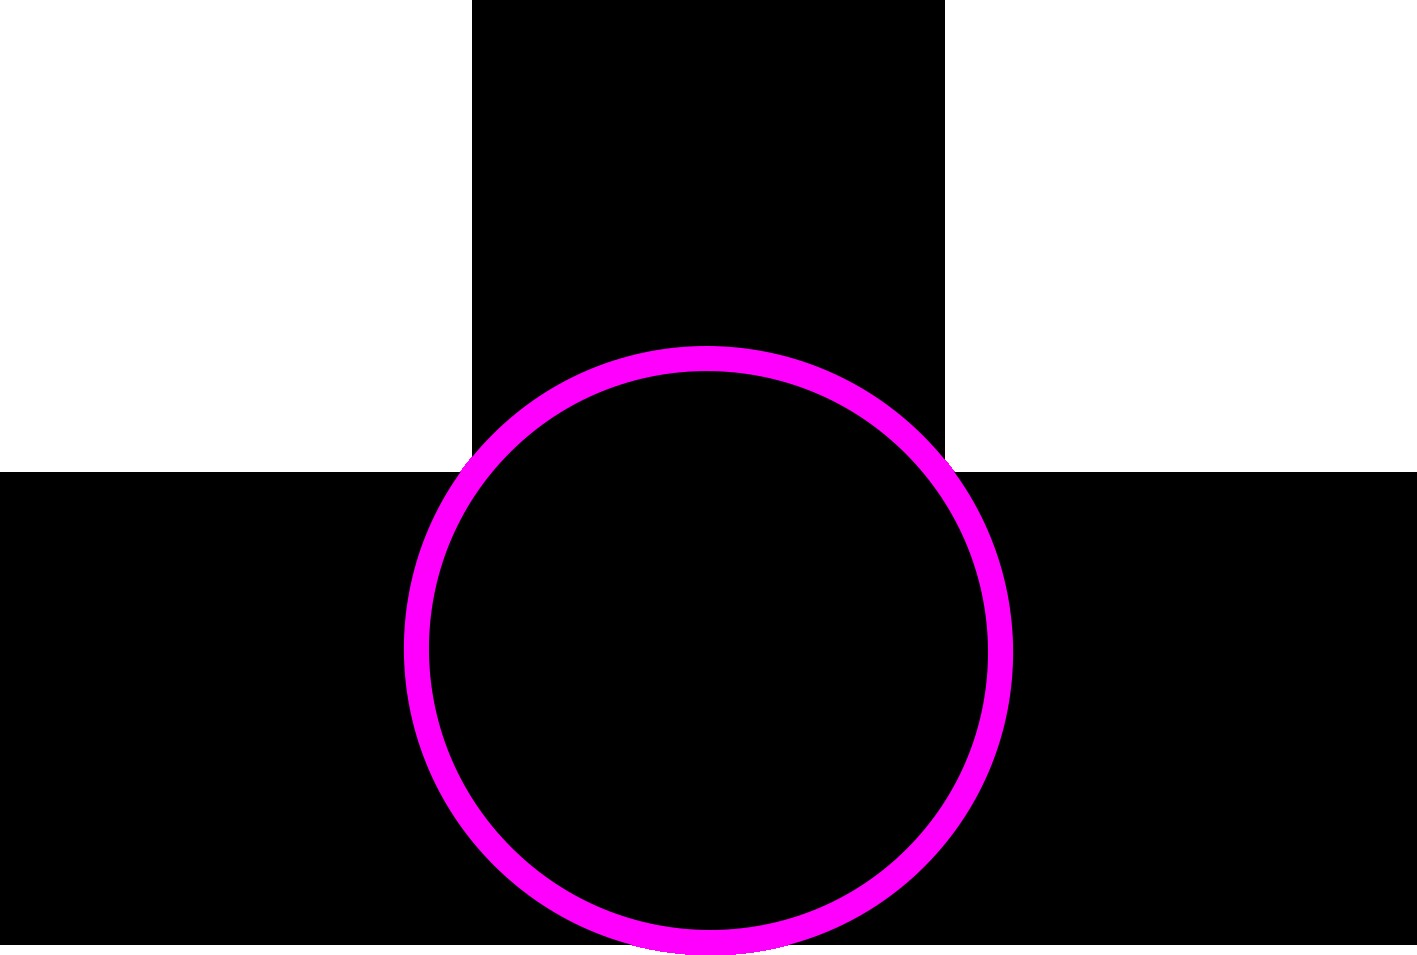
\includegraphics[width=\linewidth]{figures/circle_step_1.jpg}
            \caption{Step 1: Inscribe the largest possible circumference into the footprint geometry.}
            \label{fig:a_step_1}
        \end{subfigure} & 
        \begin{subfigure}[t]{0.2\linewidth}
            \centering
            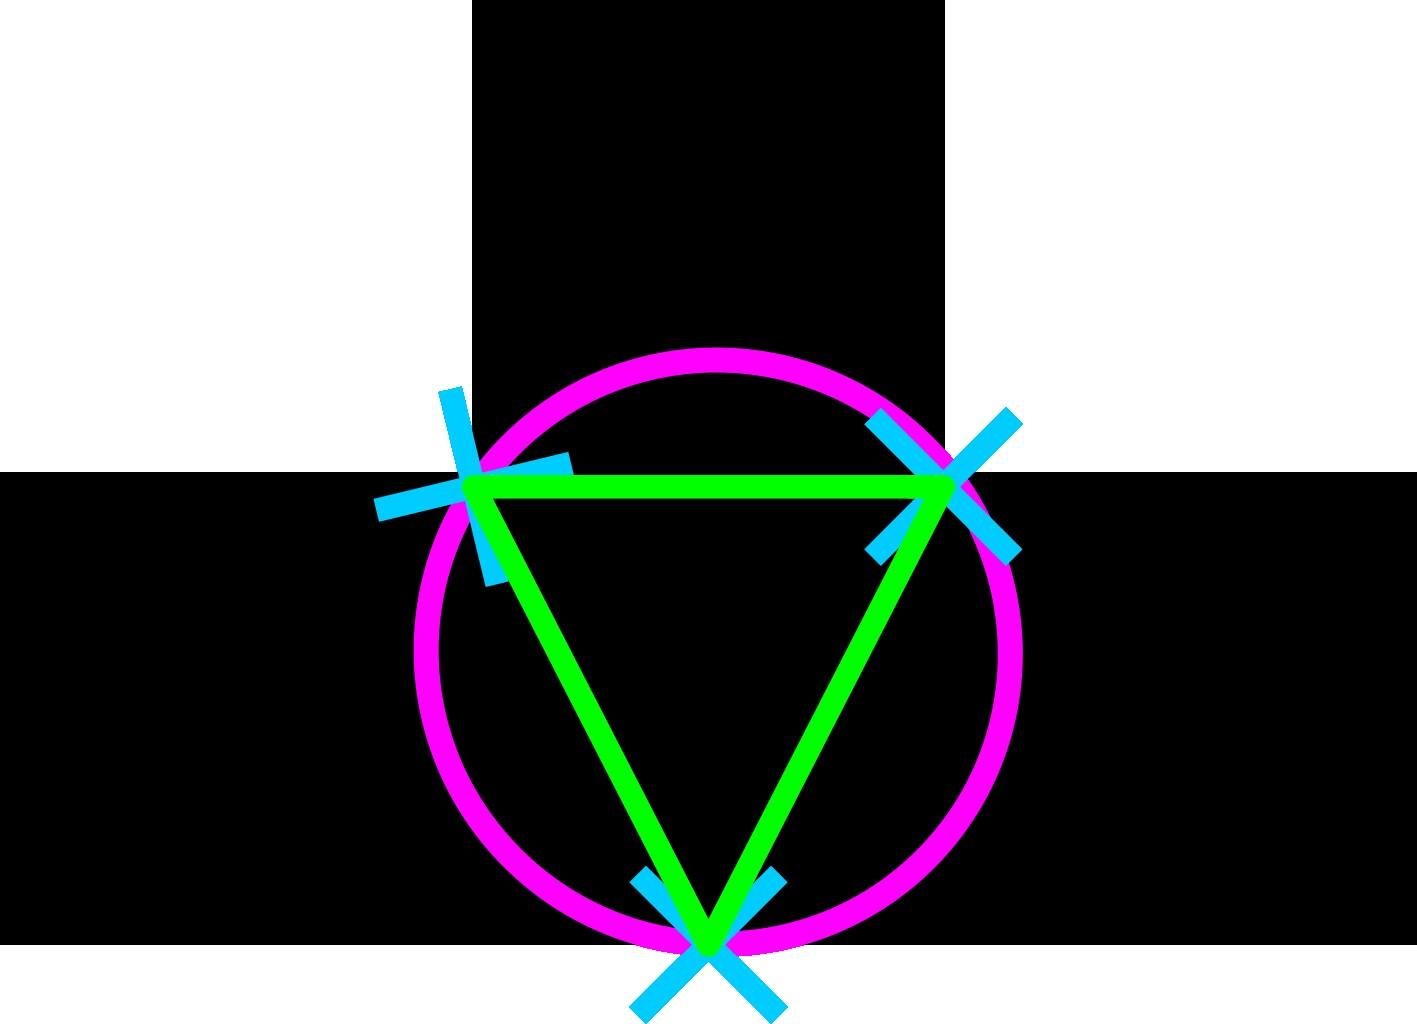
\includegraphics[width=\linewidth]{figures/circle_step_2.jpg}
            \caption{Step 2: Find the intersection points of the circumference and the footprint boundary and create a polygon.}
            \label{fig:a_step_2}
        \end{subfigure} & 
        \begin{subfigure}[t]{0.2\linewidth}
            \centering
            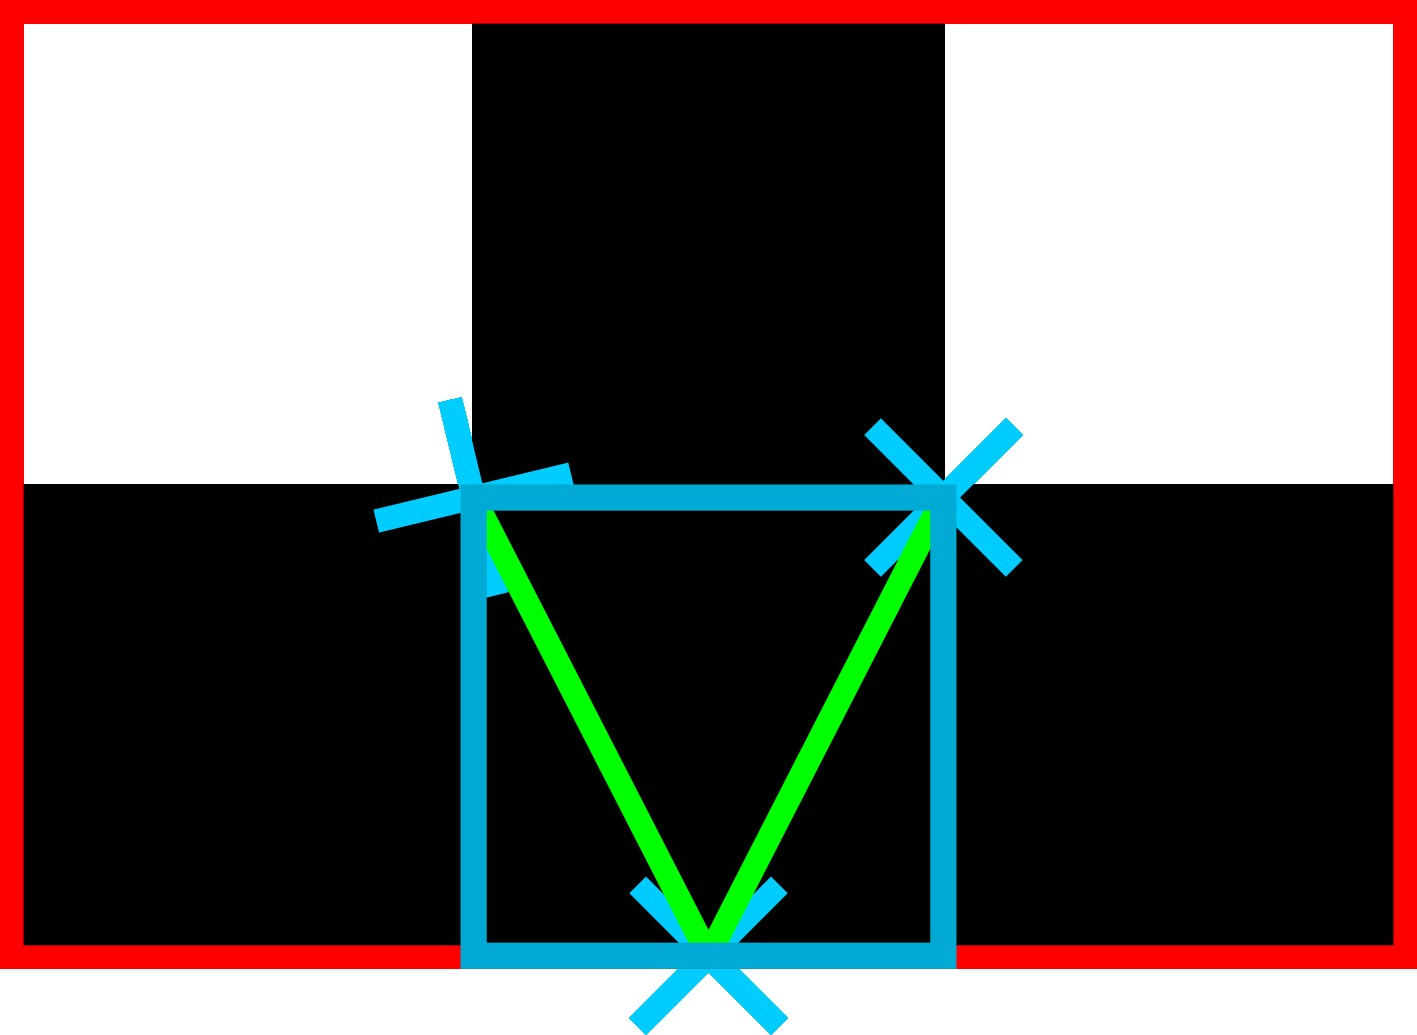
\includegraphics[width=\linewidth]{figures/circle_step_3.jpg}
            \caption{Step 3: Find the circumscribed rectangle with sides parallel to the directions of the minimum bounding box of the footprint.}
            \label{fig:a_step_3}
        \end{subfigure} & 
        \begin{subfigure}[t]{0.2\linewidth}
            \centering
            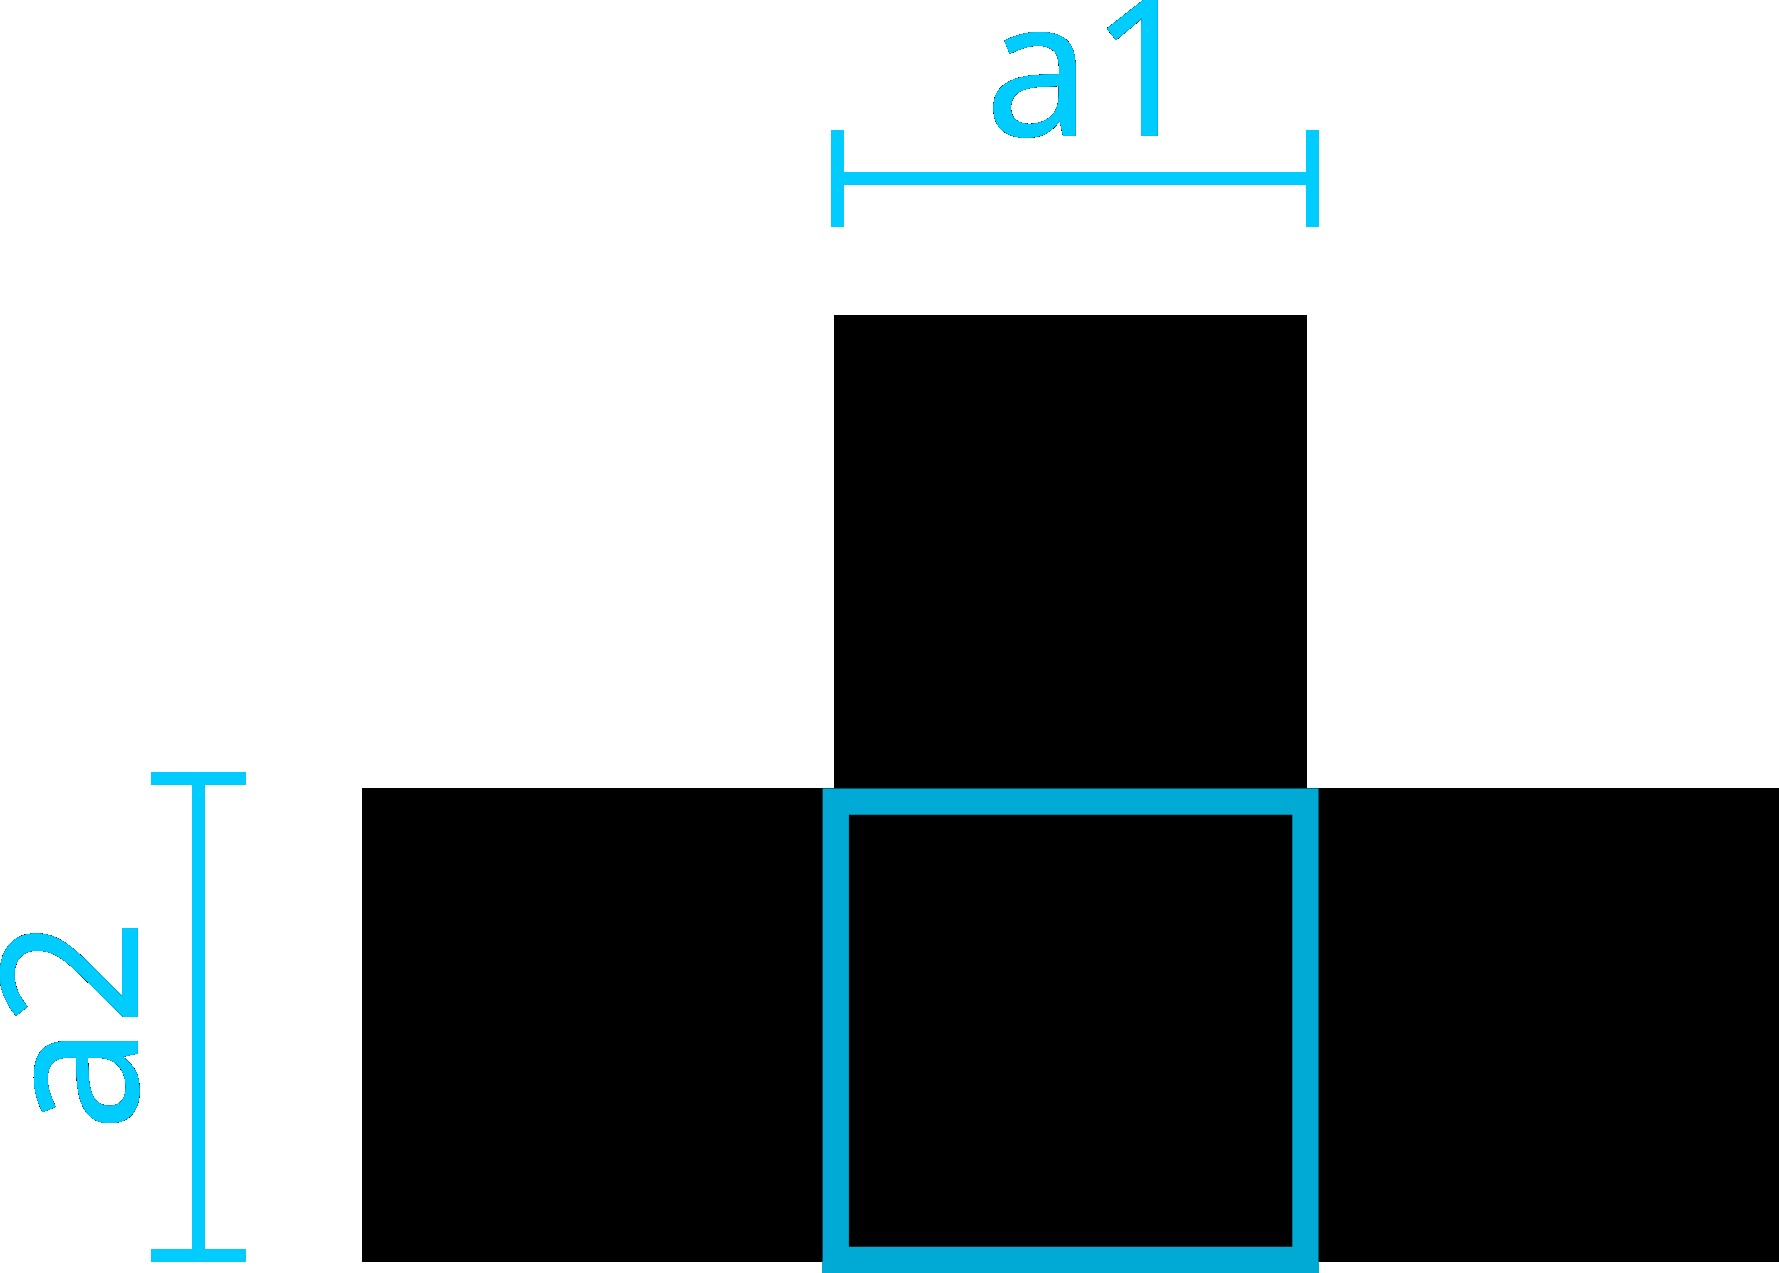
\includegraphics[width=\linewidth]{figures/circle_step_4.jpg}
            \caption{Resulting $a$ length}
            \label{fig:a_step_4}
        \end{subfigure}
    \end{tabular}
    \caption{Process to find the smallest side $a$ of the main geometric element (a rectangle) of the footprint.}
    \label{fig:process_a}
\end{figure}


\item $b$: Defined in the code as the smallest side of every setback. A setback is the set difference of the footprint geometry and its convex hull (fig \ref{fig:b_step_1}). To adapt any possible setback geometry to something with two sides a rectangle with sides parallel to the minimum bounding box of the footprint is circumscribed to every setback geometry (fig \ref{fig:b_step_2}). The sides of the setback would be the sides of the circumscribed rectangle. Setback related indices are computed for every setback returning the maximum value. 

\begin{figure}[htbp]
    \centering
    \begin{tabular}{cc}
        \begin{subfigure}[t]{0.45\linewidth}
            \centering
            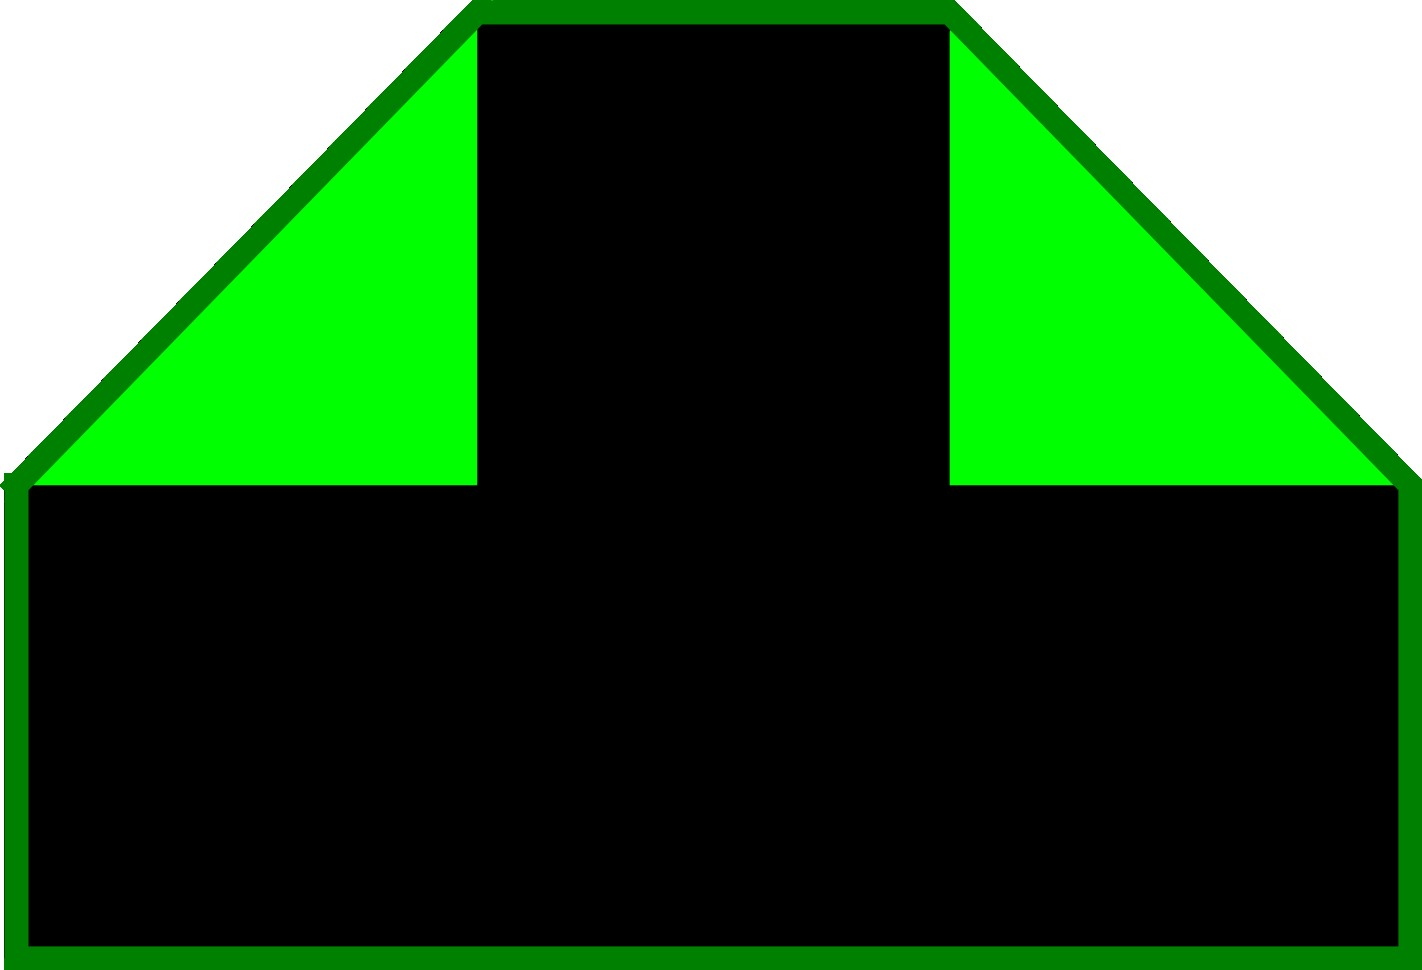
\includegraphics[width=0.6\linewidth]{figures/setback_step_1.jpg}
            \caption{Step 1: set difference of the footprint geometry (black) and its convex hull (green).}
            \label{fig:b_step_1}
        \end{subfigure} & 
        \begin{subfigure}[t]{0.45\linewidth}
            \centering
            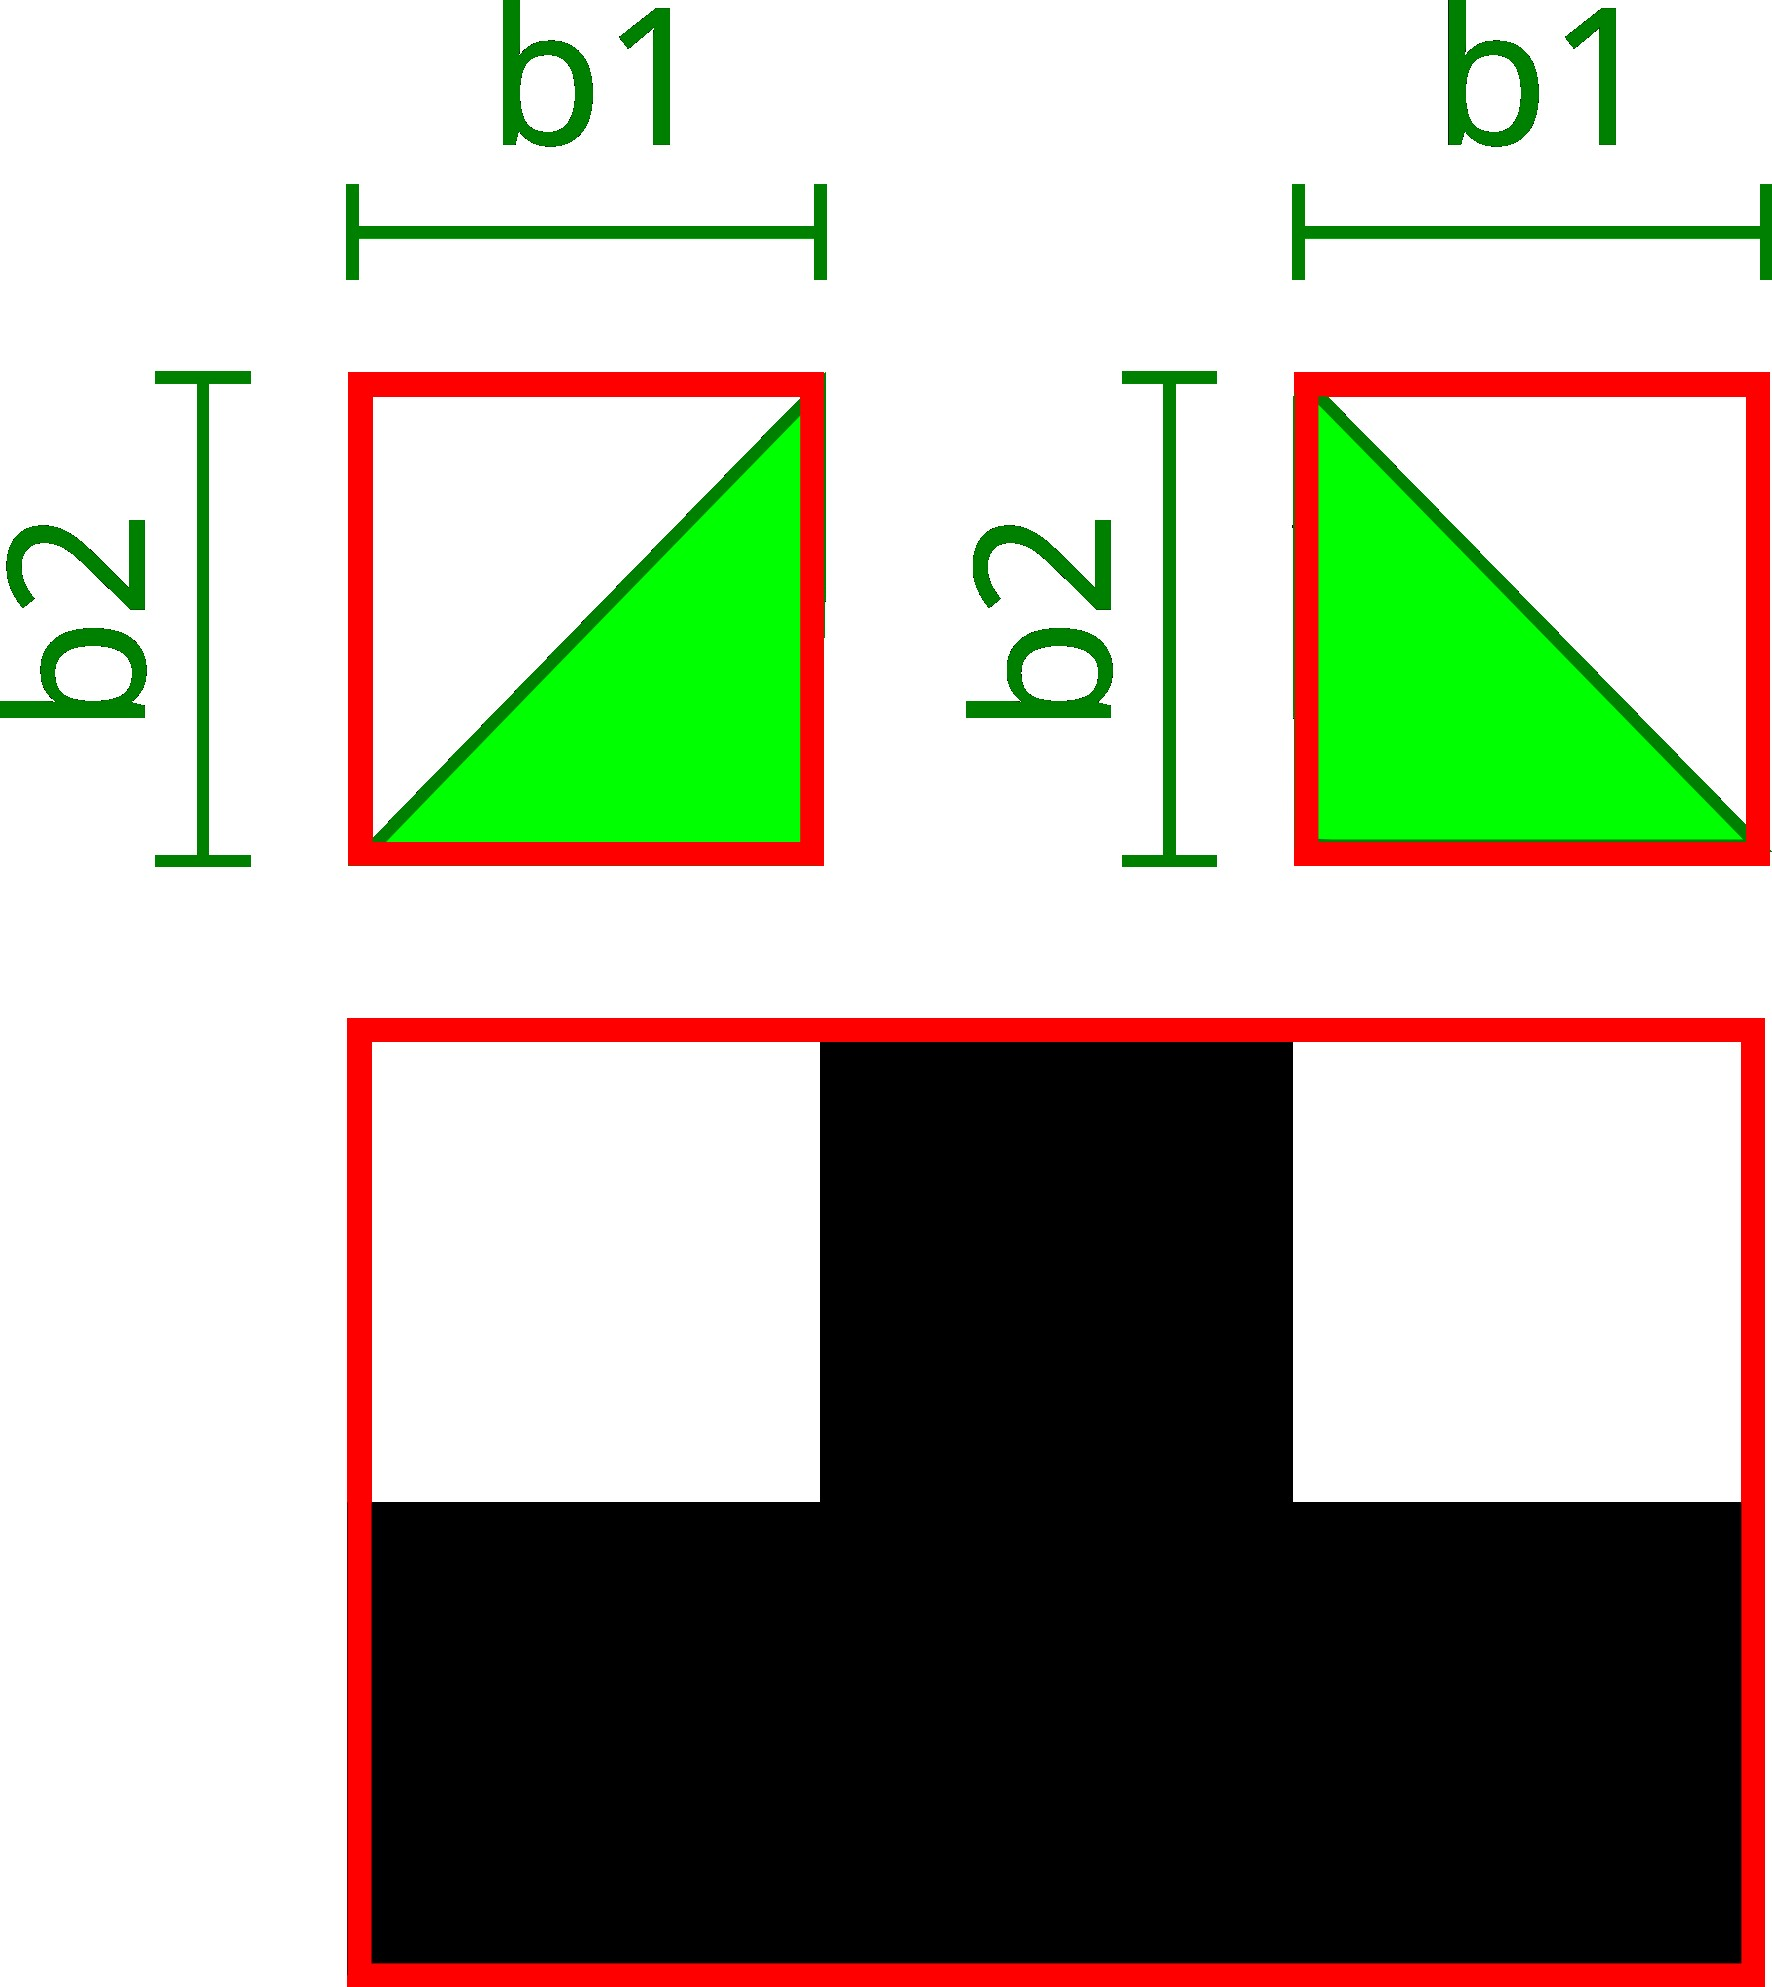
\includegraphics[width=0.6\linewidth]{figures/setback_step_2.jpg}
            \caption{Step 2: A rectangle with sides parallel to the minimum bounding box of the footprint (red) is circumscribed to every setback geometry.}
            \label{fig:b_step_2}
        \end{subfigure}
    \end{tabular}
    \caption{Process to find the setback side $b$.}
    \label{fig:process_b}
\end{figure}

\item $c$: Corresponds to the width of the footprint protrusion associated with the setback. It is measured perpendicular to $b$ using a helper line originating from the centroid of the setback geometry. 

\item $e$: Eccentricity, defined in the same way as in the Ec8 (sec \ref{sec:EC8}) as the distance between centre of mass and centre of stiffness. 
\end{itemize}


\begin{figure}[htbp]
    \centering
    \begin{tabular}{ccc}
        \begin{subfigure}[t]{0.25\linewidth}
            \centering
            
\includegraphics[width=0.6\linewidth]{figures/L_1.jpg}
            \caption{L shaped footprint).}
            \label{fig:L1}
        \end{subfigure} & 
        \begin{subfigure}[t]{0.25\linewidth}
            \centering
            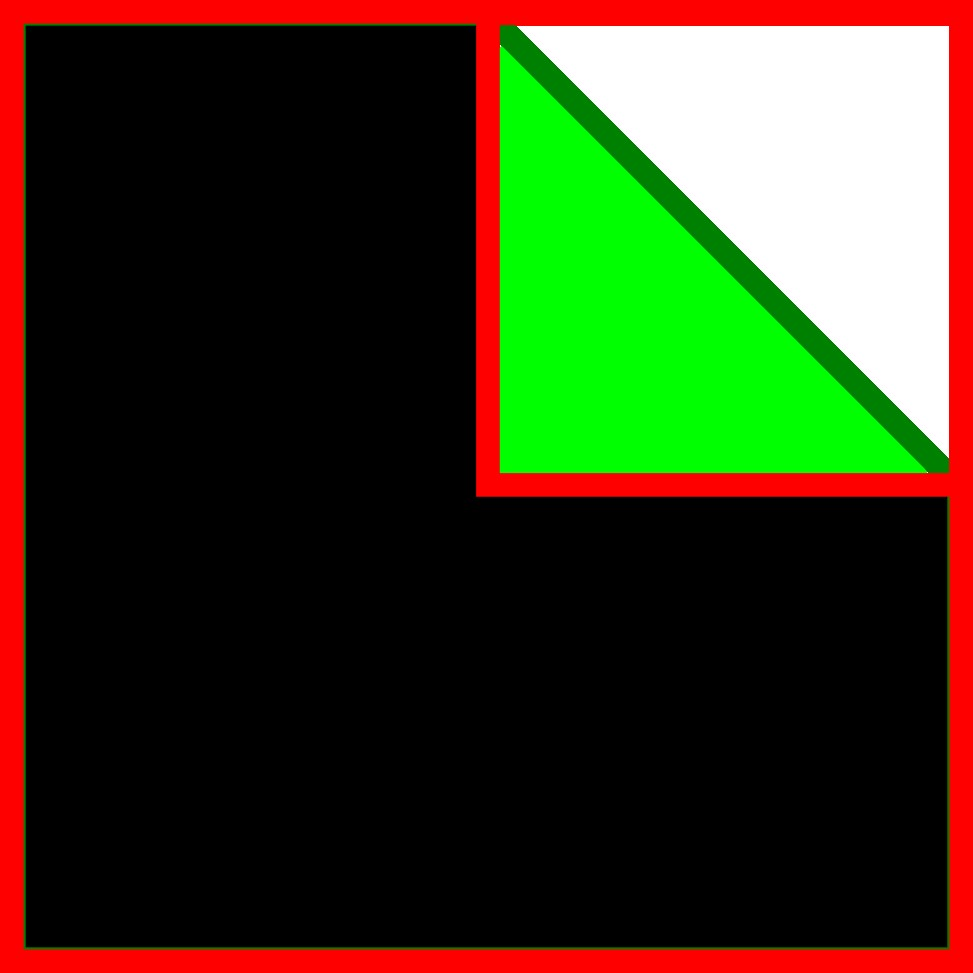
\includegraphics[width=0.6\linewidth]{figures/L_2.jpg}
            \caption{Minimum bounding box (red) and convex hull (green).}
            \label{fig:L2}
        \end{subfigure} & 
        \begin{subfigure}[t]{0.25\linewidth}
            \centering
            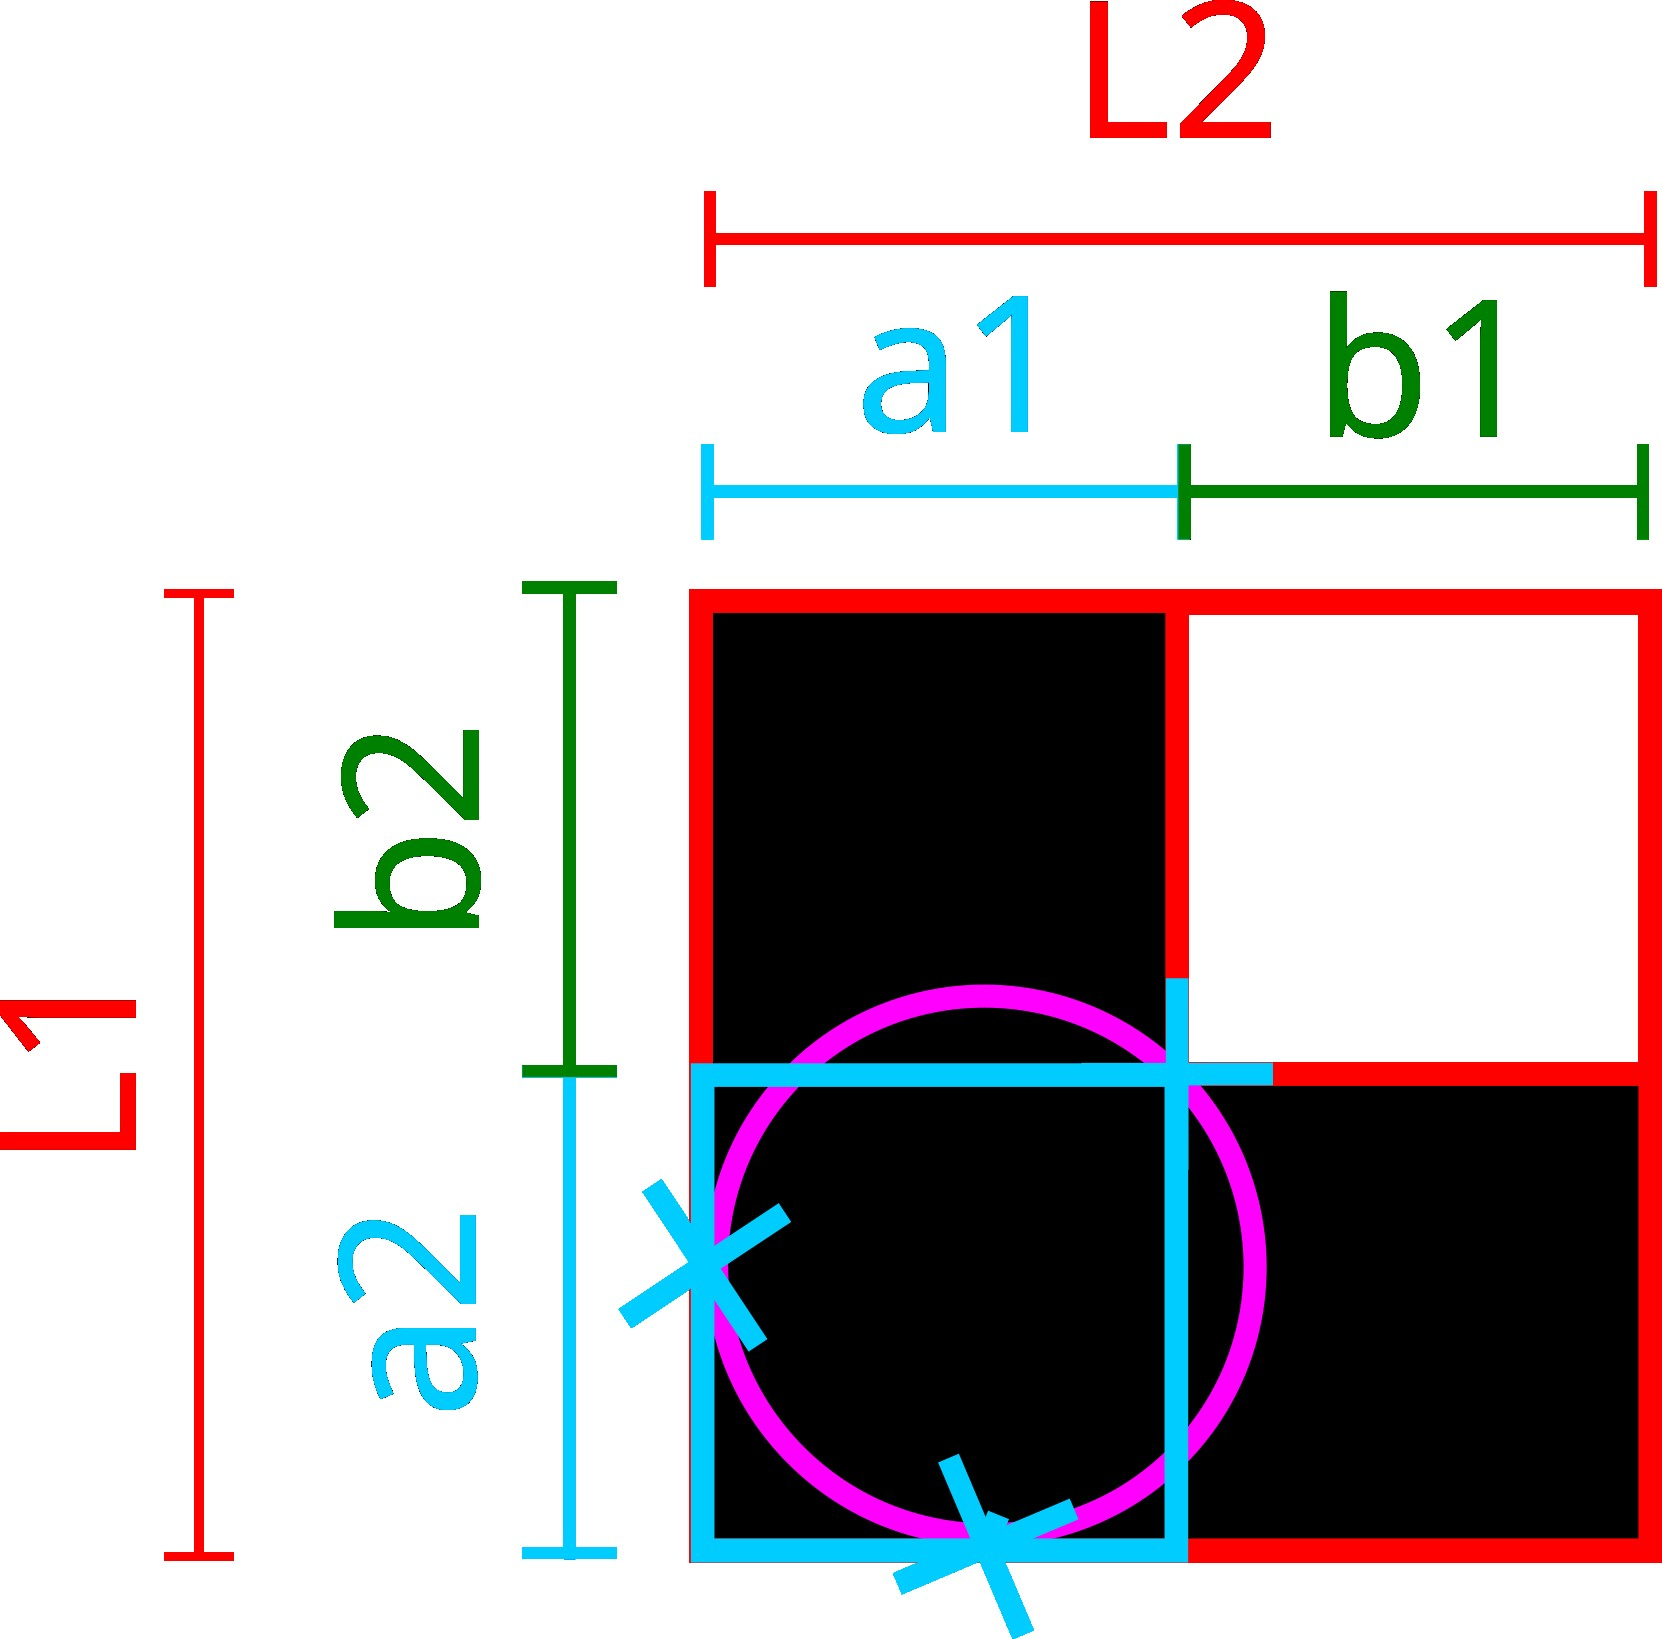
\includegraphics[width=\linewidth]{figures/L_3.jpg}
            \caption{$L$, $a$ and $b$ values computed according to figures \ref{fig:L_MBB}, \ref{fig:process_a} and \ref{fig:process_b}.}
            \label{fig:L3}
        \end{subfigure} \\
        \begin{subfigure}[t]{0.25\linewidth}
            \centering
            
\includegraphics[width=0.6\linewidth]{figures/T_1.jpg}
            \caption{T shaped footprint).}
            \label{fig:T1}
        \end{subfigure} & 
        \begin{subfigure}[t]{0.25\linewidth}
            \centering
            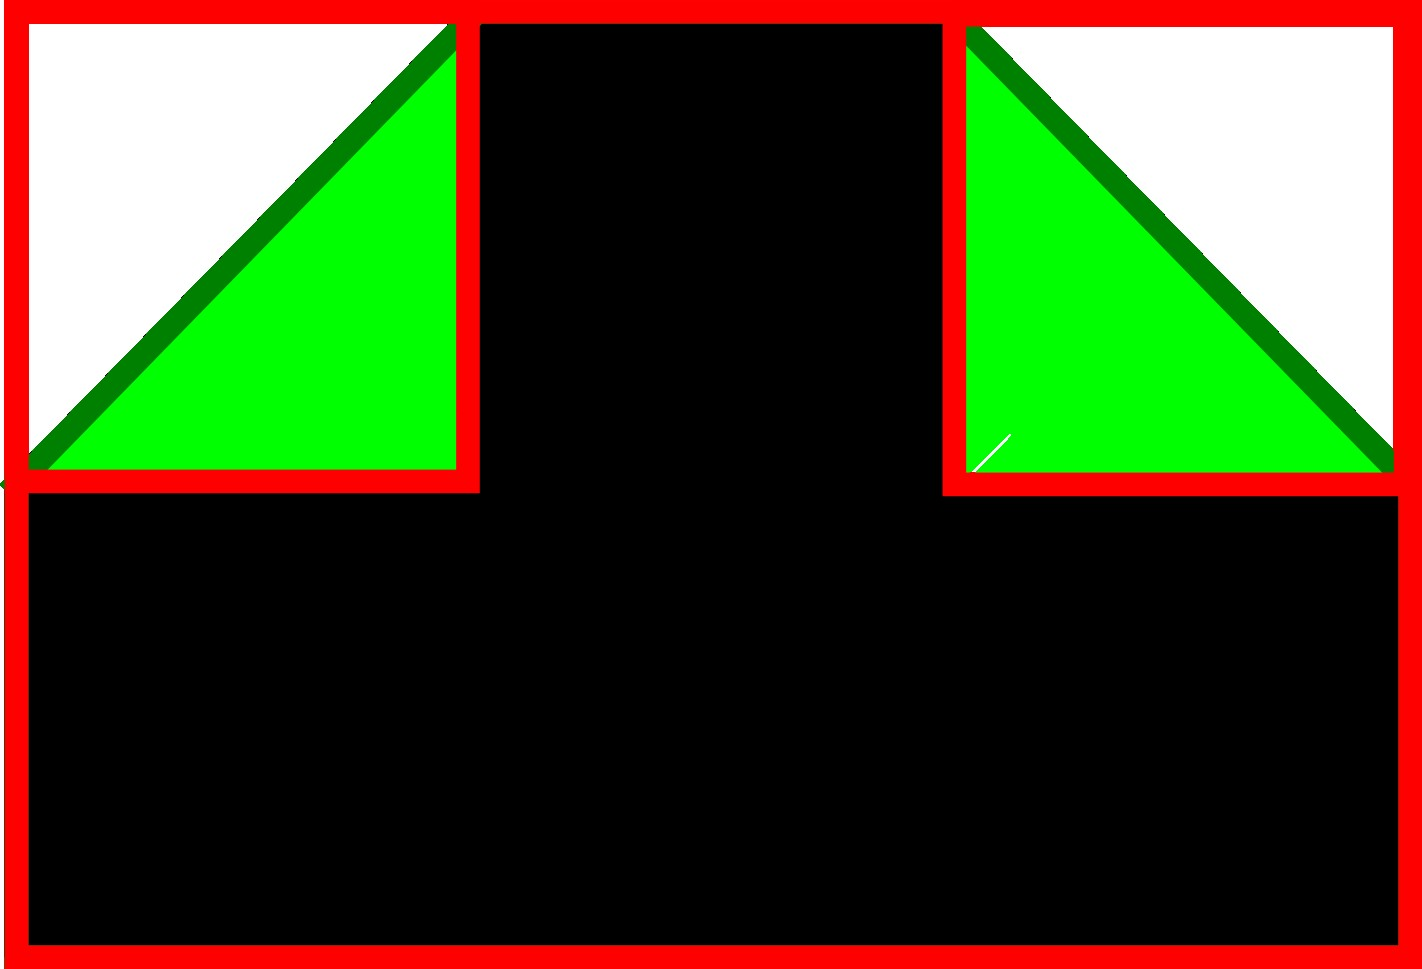
\includegraphics[width=0.6\linewidth]{figures/T_2.jpg}
            \caption{Minimum bounding box (red) and convex hull (green).}
            \label{fig:T2}
        \end{subfigure} & 
        \begin{subfigure}[t]{0.25\linewidth}
            \centering
            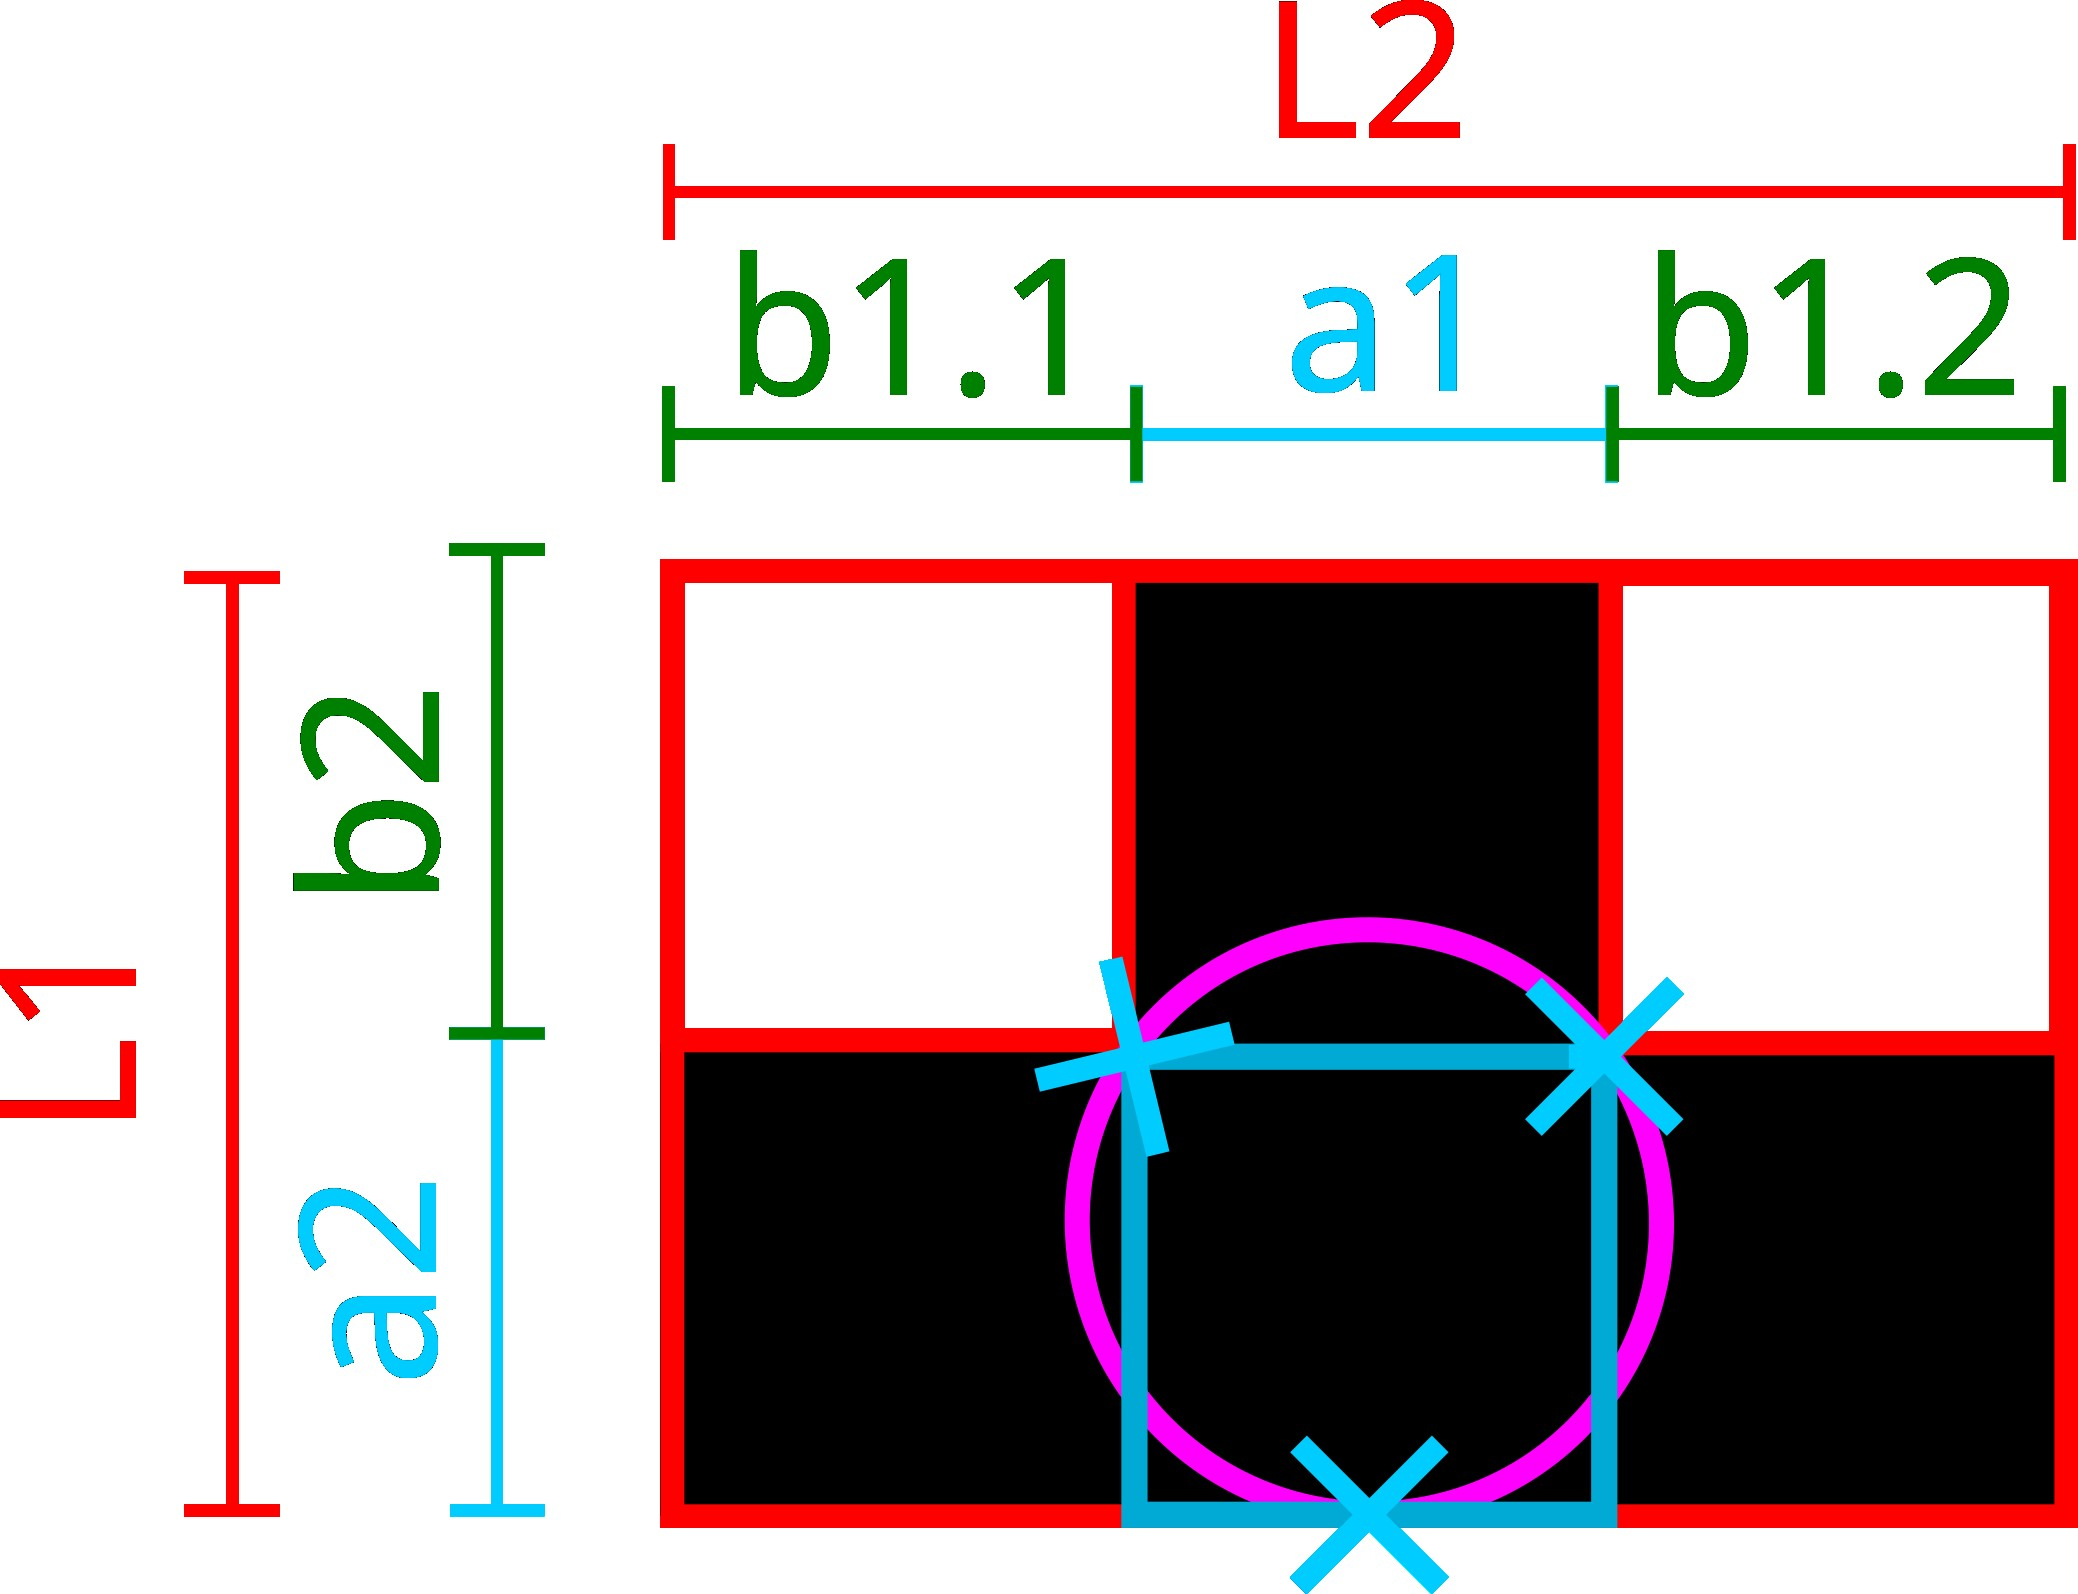
\includegraphics[width=\linewidth]{figures/T_3.jpg}
            \caption{$L$, $a$ and $b$ values computed according to figures \ref{fig:L_MBB}, \ref{fig:process_a} and \ref{fig:process_b}.}
            \label{fig:T3}
        \end{subfigure} \\
        \begin{subfigure}[t]{0.25\linewidth}
            \centering
            
\includegraphics[width=0.6\linewidth]{figures/Q_1.jpg}
            \caption{Footprint with a setback $45º$ rotated from the minimum bounding box axis.}
            \label{fig:Q1}
        \end{subfigure} & 
        \begin{subfigure}[t]{0.25\linewidth}
            \centering
            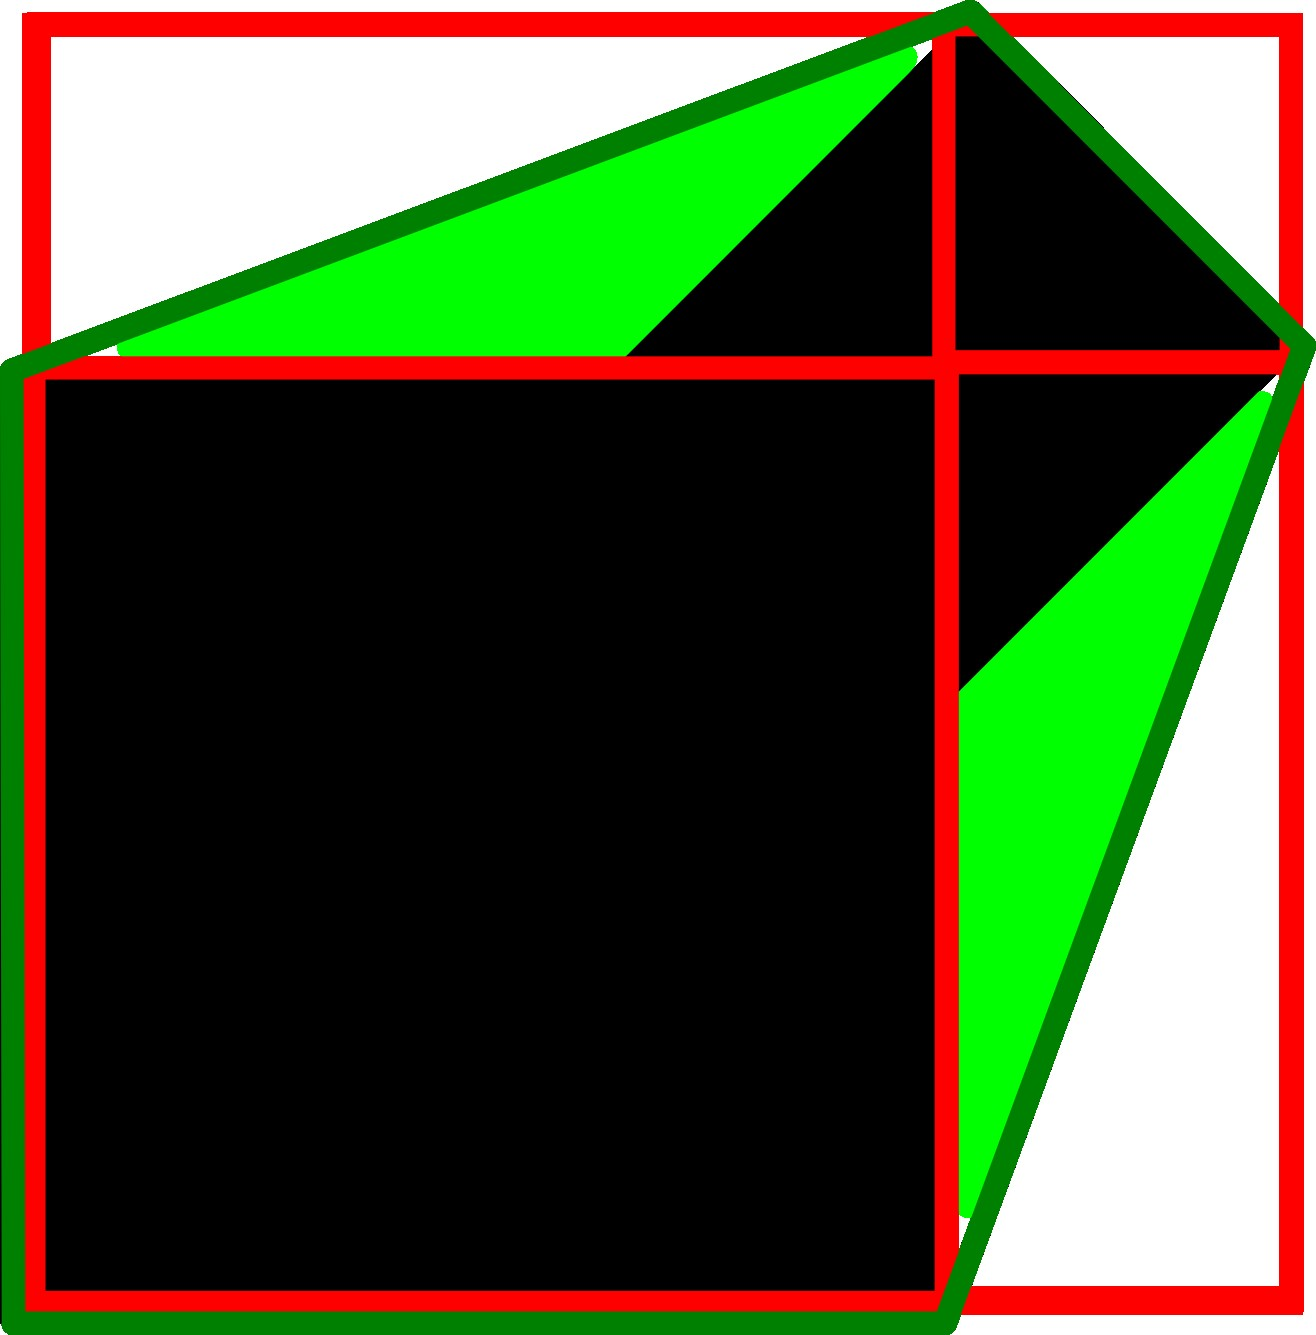
\includegraphics[width=0.6\linewidth]{figures/Q_2.jpg}
            \caption{Minimum bounding box (red) and convex hull (green).}
            \label{fig:Q2}
        \end{subfigure} & 
        \begin{subfigure}[t]{0.25\linewidth}
            \centering
            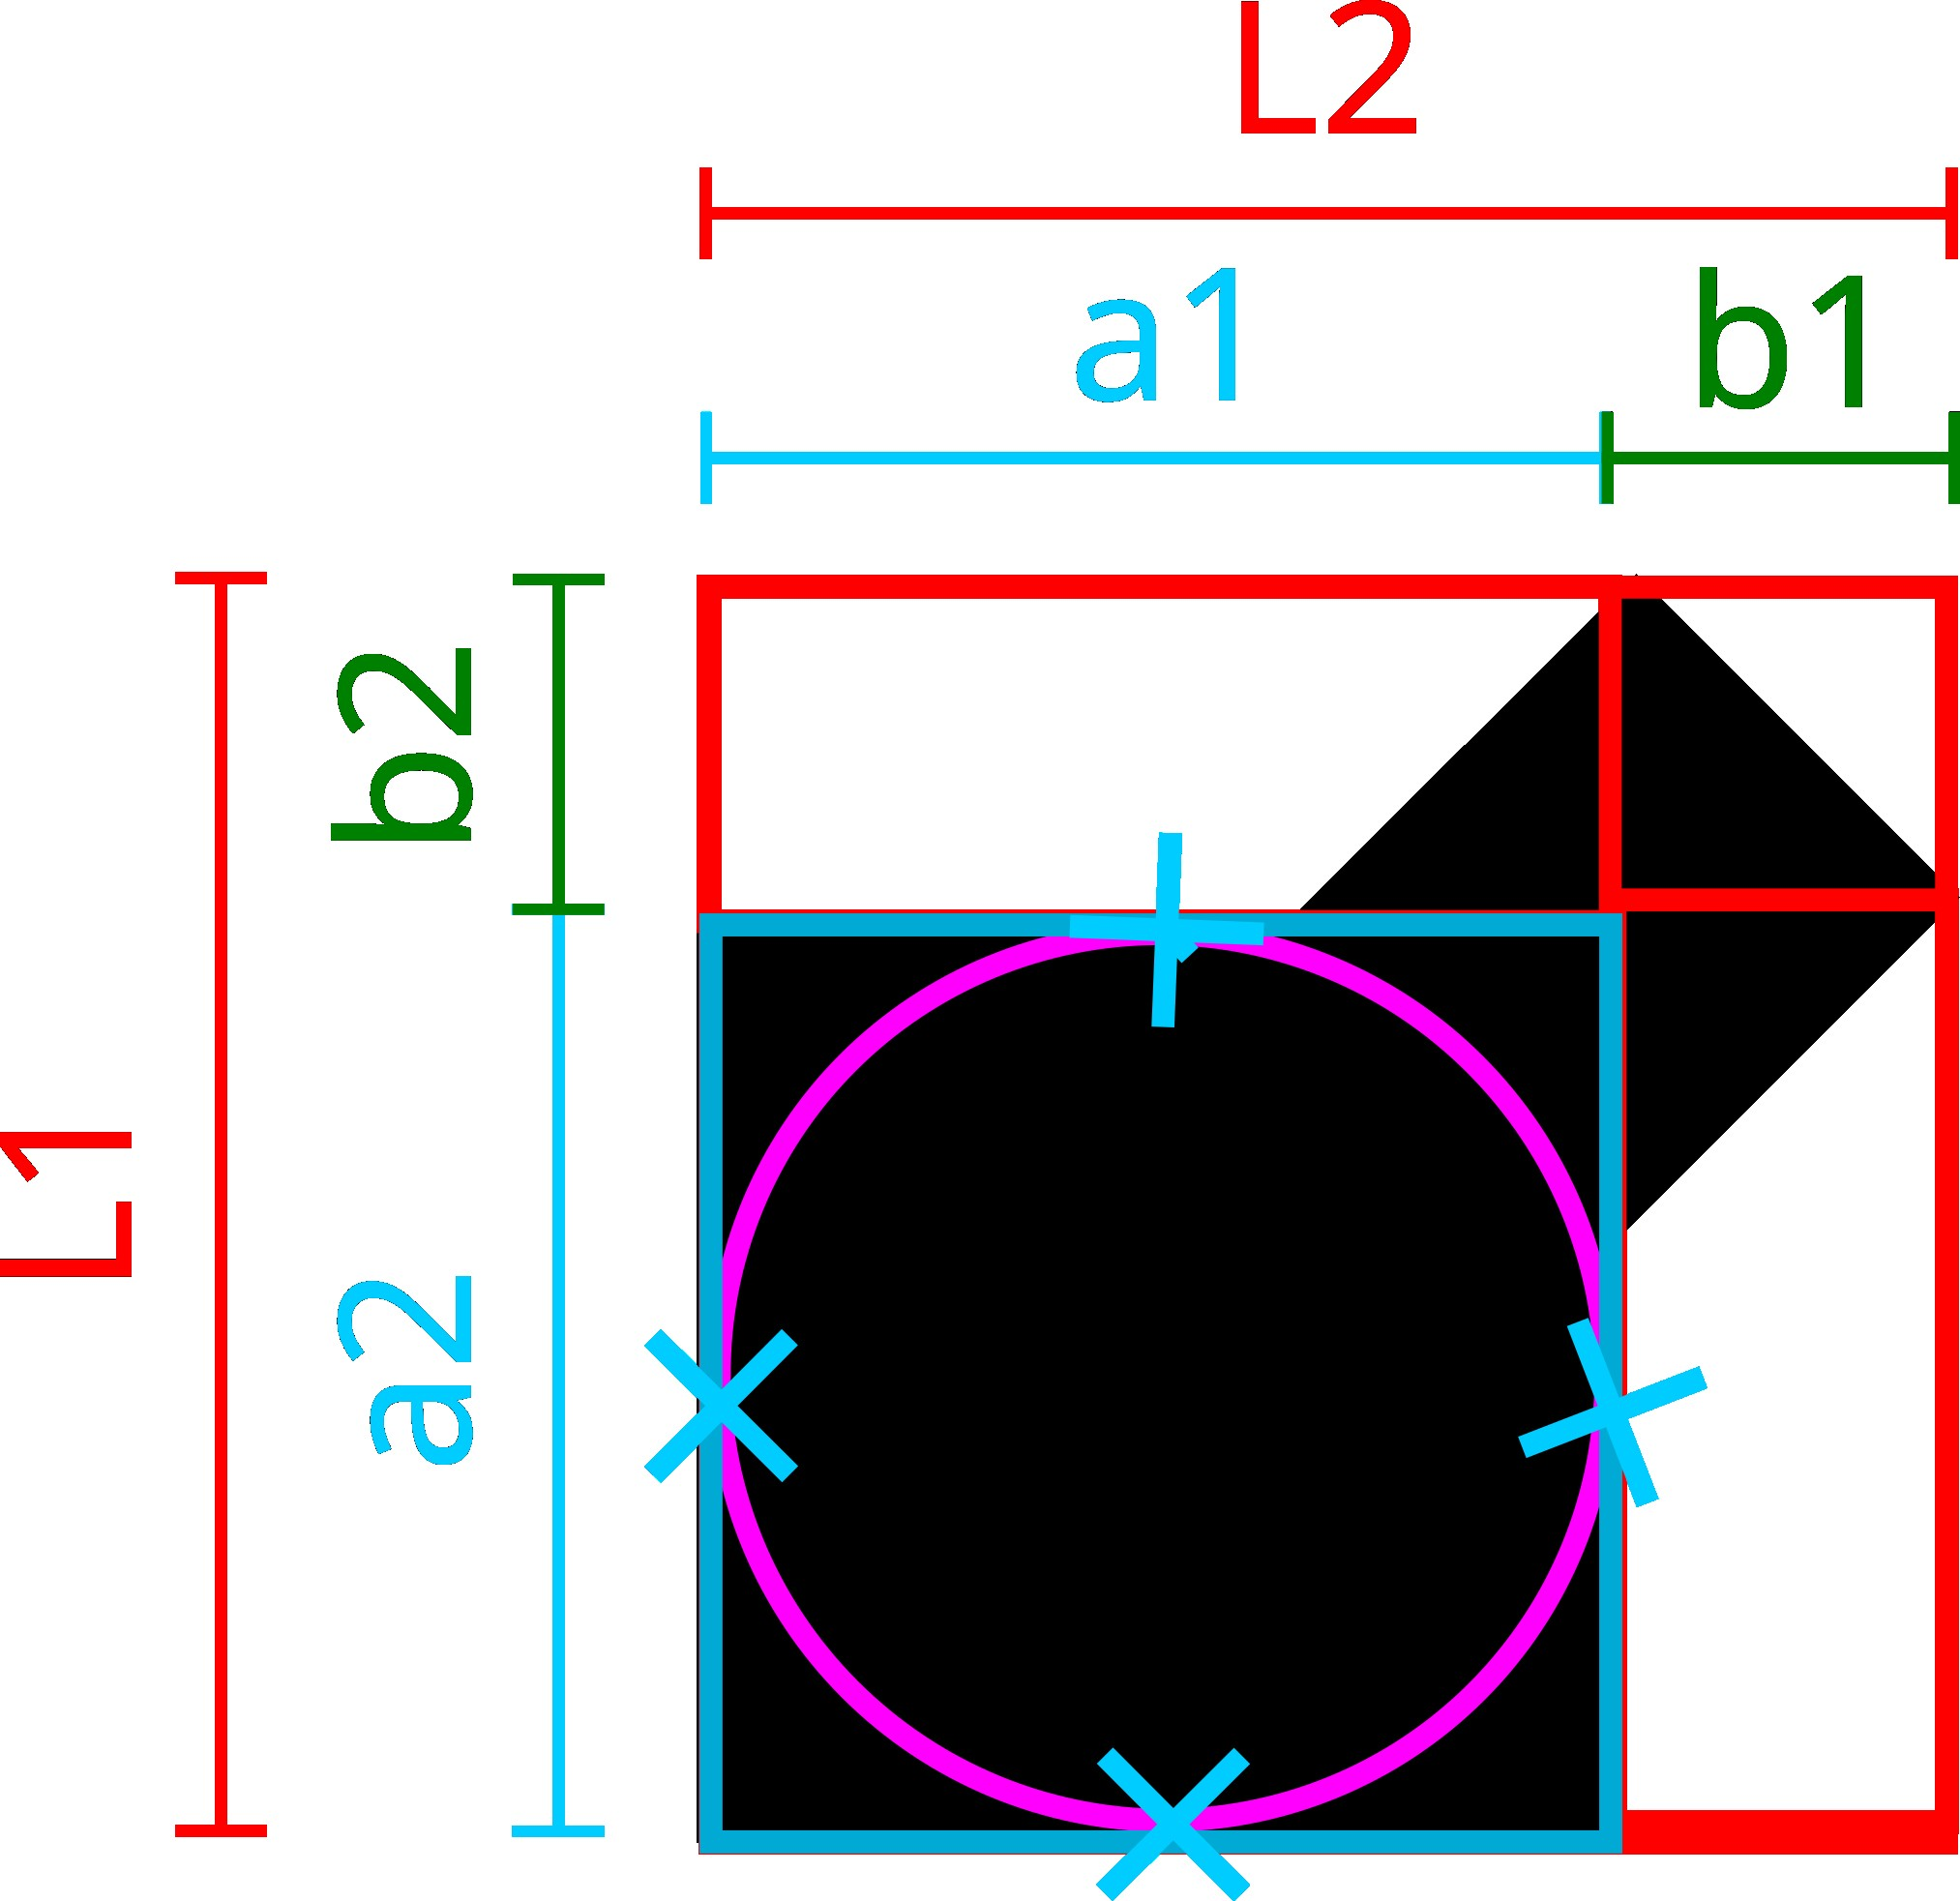
\includegraphics[width=\linewidth]{figures/Q_3.jpg}
            \caption{$L$, $a$ and $b$ values computed according to figures \ref{fig:L_MBB}, \ref{fig:process_a} and \ref{fig:process_b}.}
            \label{fig:Q3}
        \end{subfigure} \\
        \begin{subfigure}[t]{0.25\linewidth}
            \centering
            
\includegraphics[width=0.6\linewidth]{figures/LT_1.jpg}
            \caption{Triangular shaped footprint with a setback at $45º$.}
            \label{fig:LT1}
        \end{subfigure} & 
        \begin{subfigure}[t]{0.25\linewidth}
            \centering
            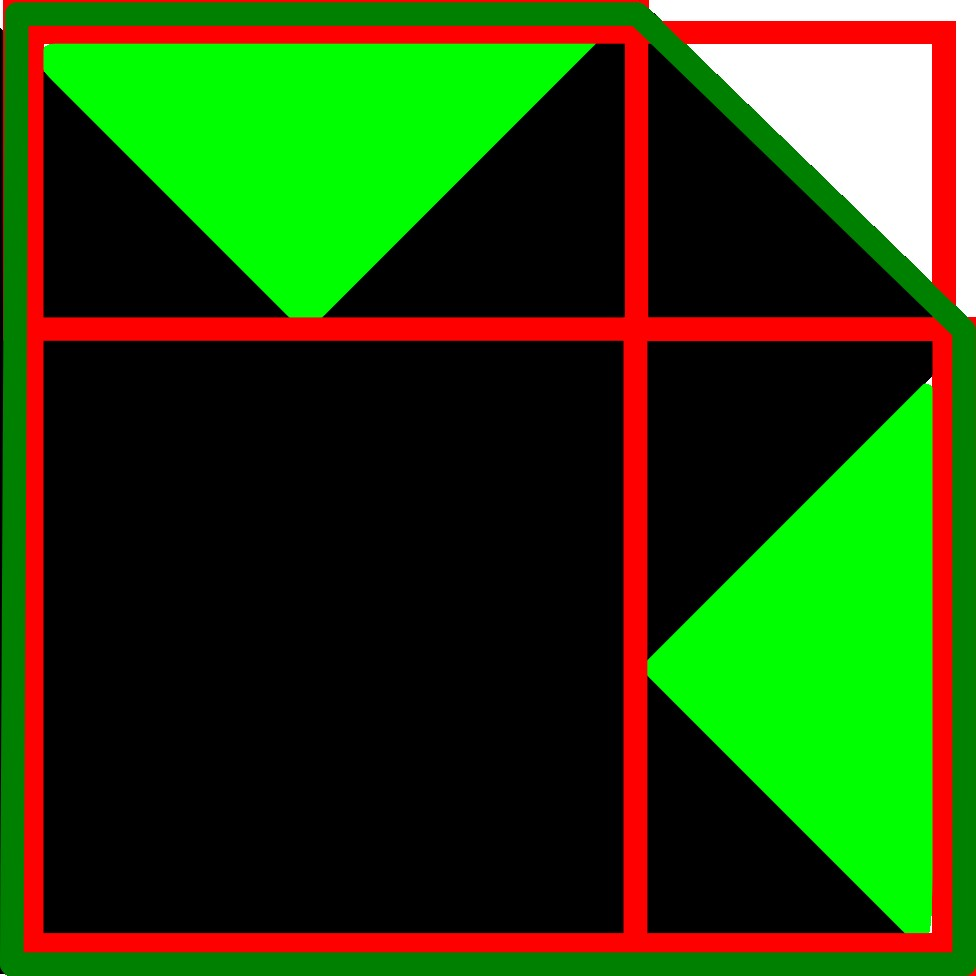
\includegraphics[width=0.6\linewidth]{figures/LT_2.jpg}
            \caption{Minimum bounding box (red) and convex hull (green).}
            \label{fig:LT2}
        \end{subfigure} & 
        \begin{subfigure}[t]{0.25\linewidth}
            \centering
            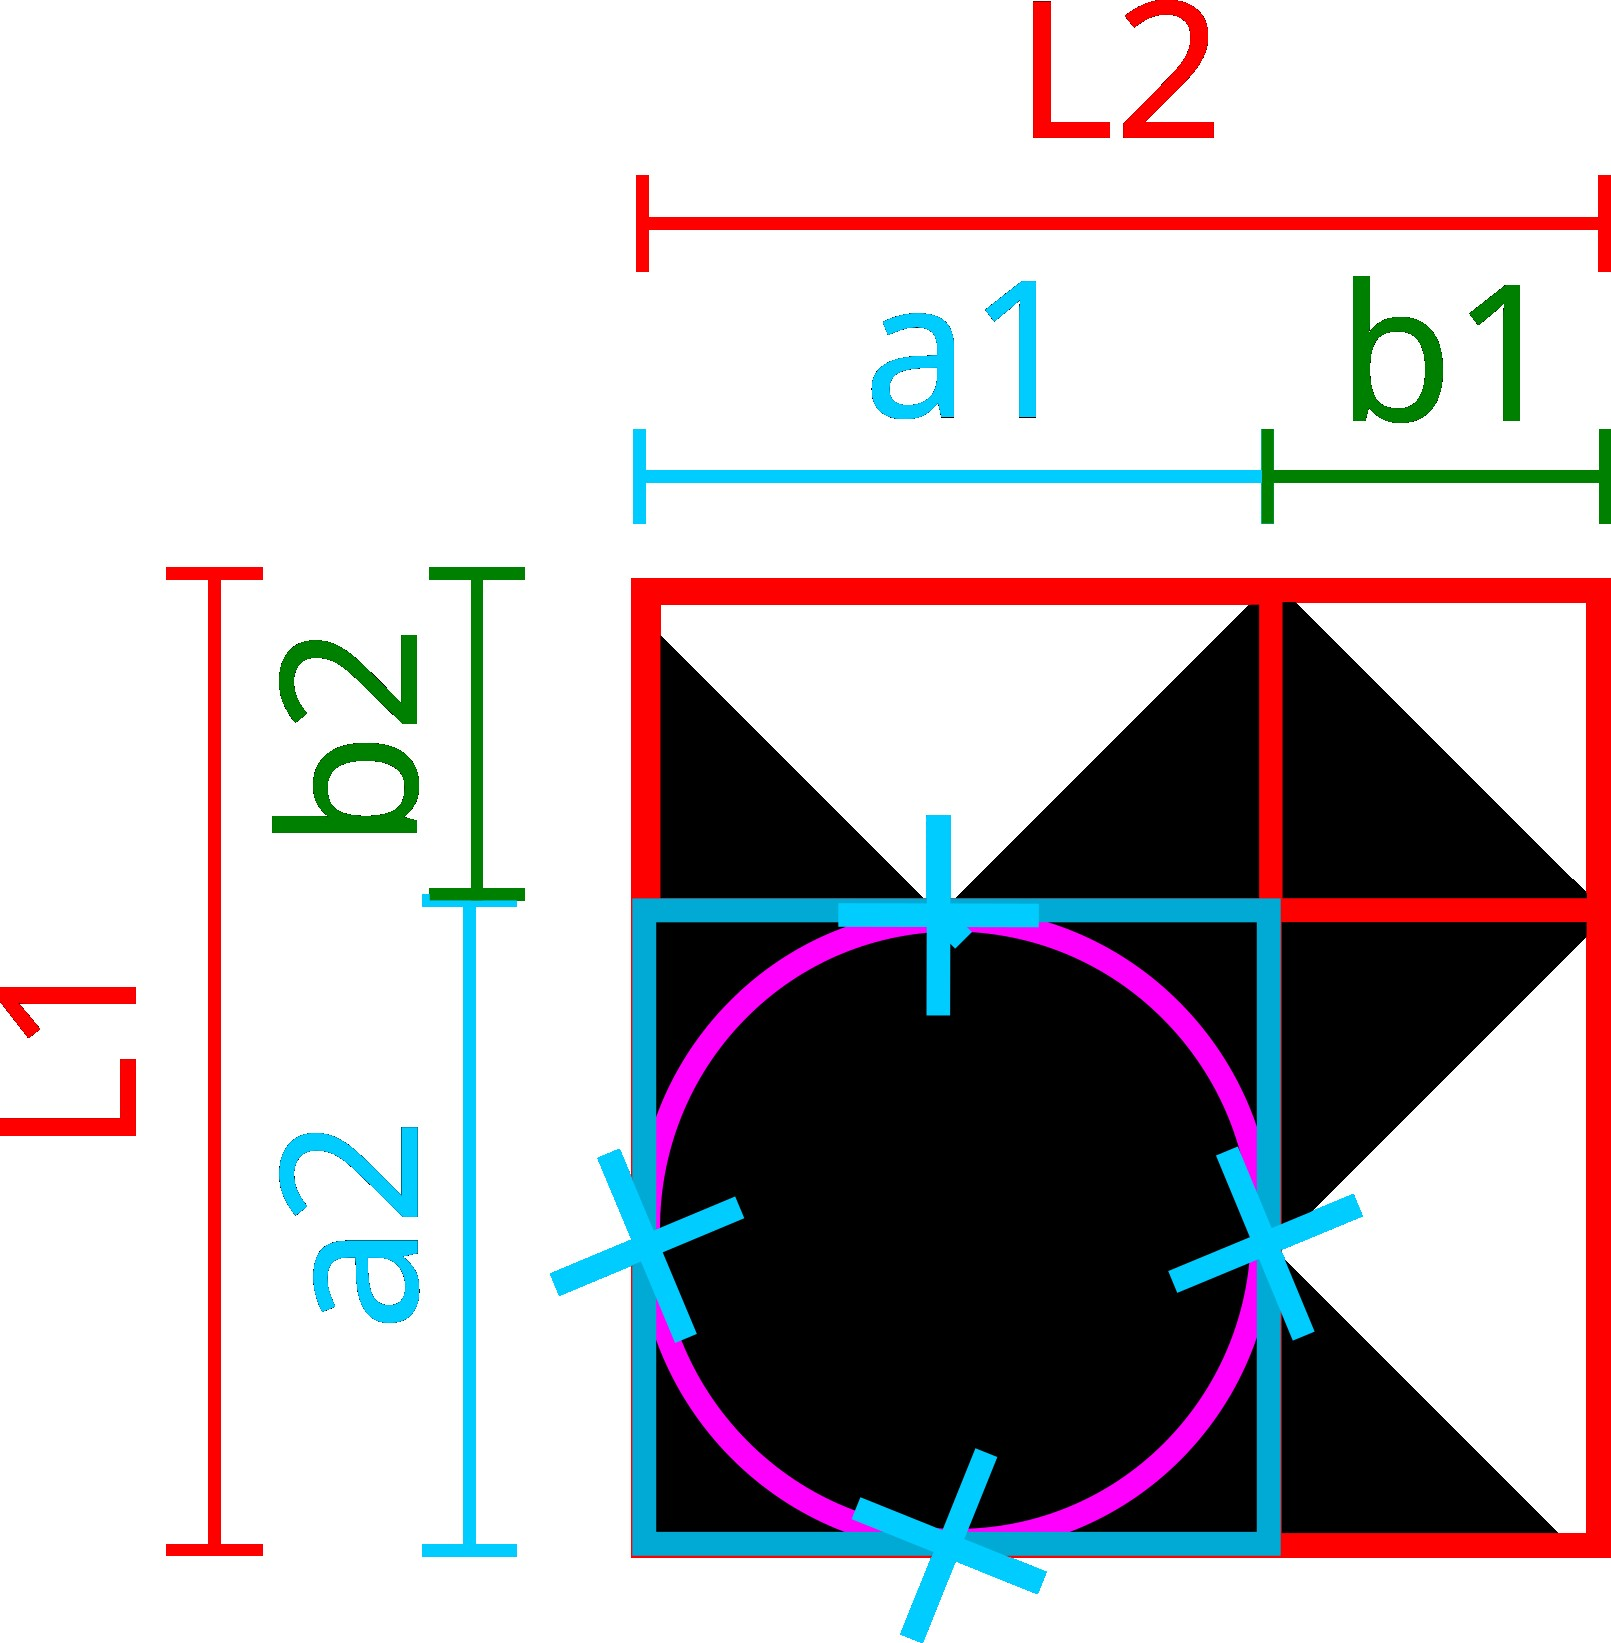
\includegraphics[width=\linewidth]{figures/LT_3.jpg}
            \caption{$L$, $a$ and $b$ values computed according to figures \ref{fig:L_MBB}, \ref{fig:process_a} and \ref{fig:process_b}.}
            \label{fig:LT3}
        \end{subfigure} \\
    \end{tabular}
    \caption{Four examples for the geometric computation process for $L$, $a$ and $b$. If the footprints has setbacks at an angle the circumscribed rectangles help finding the setback side length.}
    \label{fig:examples_GNDT}
\end{figure}


Figure \ref{fig:examples_GNDT} illustrates several examples showing how the parameters $L$, $a$, and $b$ are defined. 
In figure \ref{fig:Q2}, it is important to note that the bounding box (in red) enclosing the setbacks (in green) is not the minimum bounding box of the setback geometry itself. Instead, it is aligned parallel to the minimum bounding box of the overall building footprint. 


According to the code, the setback parameters $a$ and $b$ must be measured along the same direction, while $L$ is measured perpendicular to that direction. This results in two possible configurations for each footprint: either $(L_1, a_1, b_1)$ or $(L_2, a_2, b_2)$. The appropriate configuration is selected by choosing the one that maximizes the product \( L \cdot a \), as this identifies the dominant rectangular component in the footprint. For the parameter \( \beta_2 = \frac{b}{L} \), it is recommended to use the minimum between \( \frac{b_1}{L_1} \) and \( \frac{b_2}{L_2} \) to ensure stability, as complex setback shapes can otherwise lead to overestimated values. Taking the minimum ensures that the setback is relevant in both directions, effectively filtering out very thin or negligible setbacks.


For masonry buildings the GNDT manual defines two basic parameters, $\beta_1$ and $\beta_2$:

\begin{itemize}
    \item \textbf{Main shape slenderness} $\beta_1$ = $a$/$L$
    \item \textbf{Setback ratio} $\beta_2$ = $b$/$L$
\end{itemize}

The footprint regularity is divided into four classes with A being the best: 

\begin{itemize}
    \item \textbf{Class A}: $\beta_1 > 0.8$ and $\beta_2 < 0.1$
    \item \textbf{Class B}: $0.8 > \beta_1 > 0.6$ and $0.1 < \beta_2 < 0.2$
    \item \textbf{Class C}: $0.6 > \beta_1 > 0.4$ and $0.2 < \beta_2 < 0.3$
    \item \textbf{Class D}: $\beta_1 < 0.6$ and $\beta_2 > 0.3$
\end{itemize}

For concrete buildings, the GNDT Level II defines four fundamental parameters: $\beta_3$, $\beta_4$, $\beta_5$, and $\beta_{CR4}$. Although the original code uses different notation, the same notation adopted for masonry buildings is used here for consistency and clarity, with the inclusion of three additional parameters.

$L_1$ and $L_2$ represent the shorter and longer sides, respectively, of the building's overall footprint (fig \ref{fig:side_length}). The setback length $b$ and width $c$ is measured as previously described. Lastly, the parameter $e$ denotes the eccentricity, as defined in the Ec8 (sec \ref{sec:EC8}).


\begin{itemize}
    \item \textbf{Footprint slenderness} $\beta_3$ = $L_2$/$L_1$ Equivalent to the slenderness defined in the Ec8 (sec \ref{sec:EC8}).
    \item \textbf{Eccentricity ratio} $\beta_4$ = $e$/$a$
    \item \textbf{Cantilever ratio} $\beta_5$ = $\Delta a$/$a$, where $\Delta a$ is the width of the cantilevered elements, like balconies. This parameter cannot be estimated directly from the footprint without any additional information.
    \item \textbf{Setback slenderness} $\beta_6$ = $c$/$b$, the slenderness of the setbacks bounding box.
\end{itemize}

The footprint regularity is divided into three classes with A being the best: 

\begin{itemize}
    \item \textbf{Class A}: $\beta_3 > 0.4$ and $\beta_4 < 0.2$, at least $70\%$ of the cantilevered elements with $\beta_5 < 0.2$ and all setbacks with $\beta_6 > 0.5$.
    \item \textbf{Class B}: All footprints that are neither A nor C
    \item \textbf{Class C}: One of the following conditions: 
    \begin{itemize}
        \item $\beta_3 < 0.2$ and more than $30\%$ of the cantilevered elements surpass $\beta_5 > 0.2$
        \item $\beta_4 > 0.4$
        \item More than $70\%$ of the cantilevered elements surpass $\beta_5 > 0.2$
        \item At least one setback with $\beta_6 < 0.25$
    \end{itemize}
\end{itemize}

This study introduces regularity classes, as defined in table \ref{tab:GNDT_limits}, to standardise seismic vulnerability assessments for both masonry and reinforced concrete buildings during the preliminary design phase. These classes evaluate structural configuration and construction quality, assigning numerical values to key parameters. The resulting vulnerability index facilitates consistent risk comparisons in different building typologies. This approach is particularly useful when the structural system is not yet fully defined.


\begin{table}[htbp]
\centering
\caption{Classification criteria for masonry and concrete buildings adapted from the GNDT manual.}
\label{tab:GNDT_limits}
\begin{tabular}{|l|ccccccccc|}
\hline
\textbf{Class} & $\beta_1$ & & $\beta_2$ & & $\beta_3$ & & $\beta_4$ & & $\beta_6$ \\
\hline
A & $> 0.8$ & & $< 0.1$ & & $> 0.4$ & & $< 0.2$ & & $> 0.5$ \\
\hline
B & $> 0.6$ & & $< 0.2$ & & $> 0.2$ & & $< 0.4$ & & $> 0.25$ \\
\hline
C & $> 0.4$ & & $< 0.3$ & & $> 0.2$ & & $< 0.4$ & & $> 0.25$ \\
\hline
D & $< 0.4$ & \textit{or} & $> 0.3$ & \textit{or} & $< 0.2$ &  \textit{or} & $> 0.4$ & \textit{or} & $< 0.25$\\
\hline
\end{tabular}
\end{table}

\FloatBarrier

\renewcommand{\sectionnametext}{ASCE 7 Code}
\renewcommand{\headingtextR}{\thesection. \sectionnametext}
\section{\sectionnametext}

The ASCE 7 code \footcite{asce_american_society_of_civil_engineers_minimum_2021} includes setback-related indices analogous to those defined in the GNDT code. While it is a U.S. based norm, it has seen broad application across various countries in the Americas. It also accounts for openings (holes) in the building footprint and qualitatively identifies nonparallel sides and triangular-shaped footprints as unfavourable for seismic performance, although it does not specify quantitative thresholds. Other irregularity indices, not limited to the footprint and not addressed in this paper, include diaphragm rigidity irregularities, wall offsets, and torsional displacements.

\begin{itemize}
    \item \textbf{Setback Ratio}: This index is calculated following equation \ref{eq:setback_ratio}.
    \begin{equation} 
        \label{eq:setback_ratio}
        \text{setback\_ratio} = \frac{b}{L}
    \end{equation}
    The setback ratio should reflect the worst-case scenario across both directions and all potential setbacks. Setbacks can introduce weak points at corners, especially when they cause localized changes in vibration modes.

    The computation of the setback ratio aligns with the Italian GNDT code, with modifications to the sides used in the formula as illustrated in figure \ref{fig:NTC_setback_ratio}. The setback ratio is set to the minimum of $b1/L1$ and $b2/L2$. Taking the minimum ensures that the setback is relevant in both directions, effectively filtering out very thin or negligible setbacks.

    \item \textbf{Hole Ratio}: Defined by equation \ref{eq:hole_ratio_a}, this ratio measures the proportion of hole area to the total area of the footprint assuming all holes are filled. Holes are defined as the set difference between the area of the footprint polygon with all holes filled and the actual footprint polygon including holes.
    \begin{equation}
        \label{eq:hole_ratio_a}
        \text{hole\_ratio} = \frac{A_{\text{hole}}}{A_{\text{filled}}}    
    \end{equation}
    
    \item \textbf{Parallelity Angle}: This index quantifies how aligned the sides of the footprint are with respect to a reference rectangular bounding box. While the ASCE 7 code suggests avoiding triangular shapes, it does not provide a quantitative measure. In this paper, a new index is proposed: for each edge of the footprint, the minimum angle between that edge and any side of the minimum bounding box is calculated. These angles are then averaged, weighted by the corresponding edge lengths (eq \ref{eq:paralelity_angle}). A mean angle exceeding 5–10 degrees typically indicates a triangular footprint.
    \begin{equation}
        \label{eq:paralelity_angle}
        \text{parallelity\_angle} = \frac{\sum l_i \cdot \min\left(\angle(l_i,\text{mbox}_1),\angle(l_i,\text{mbox}_2)\right)}{\sum l_i}    
    \end{equation}
\end{itemize}


The code limits parameters according to table \ref{tab:asce_limits}.

\begin{table}[htbp]
    \centering
    \caption{Limitations of each irregularity parameter according to the ASCE 7 code.}
    \begin{tabular}{|c|c|}
        \hline
        \textbf{Parameter} & \textbf{Limit}\\
        \hline
        \textbf{Setback ratio} & $\leq 0.2$\\
        \hline
        \textbf{Hole ratio}  & $\leq 0.25$\\
        \hline
        \textbf{Parallelity Angle}  & No triangular shapes\\
        \hline
    \end{tabular}
    \label{tab:asce_limits}
\end{table}

\FloatBarrier

\renewcommand{\sectionnametext}{NTC-23 seismic code for Mexico city}
\renewcommand{\headingtextR}{\thesection. \sectionnametext}
\section{\sectionnametext}

\begin{figure}[htbp]
    \centering
    \begin{tabular}{cc}
        \begin{subfigure}[t]{0.3\linewidth}
            \centering
            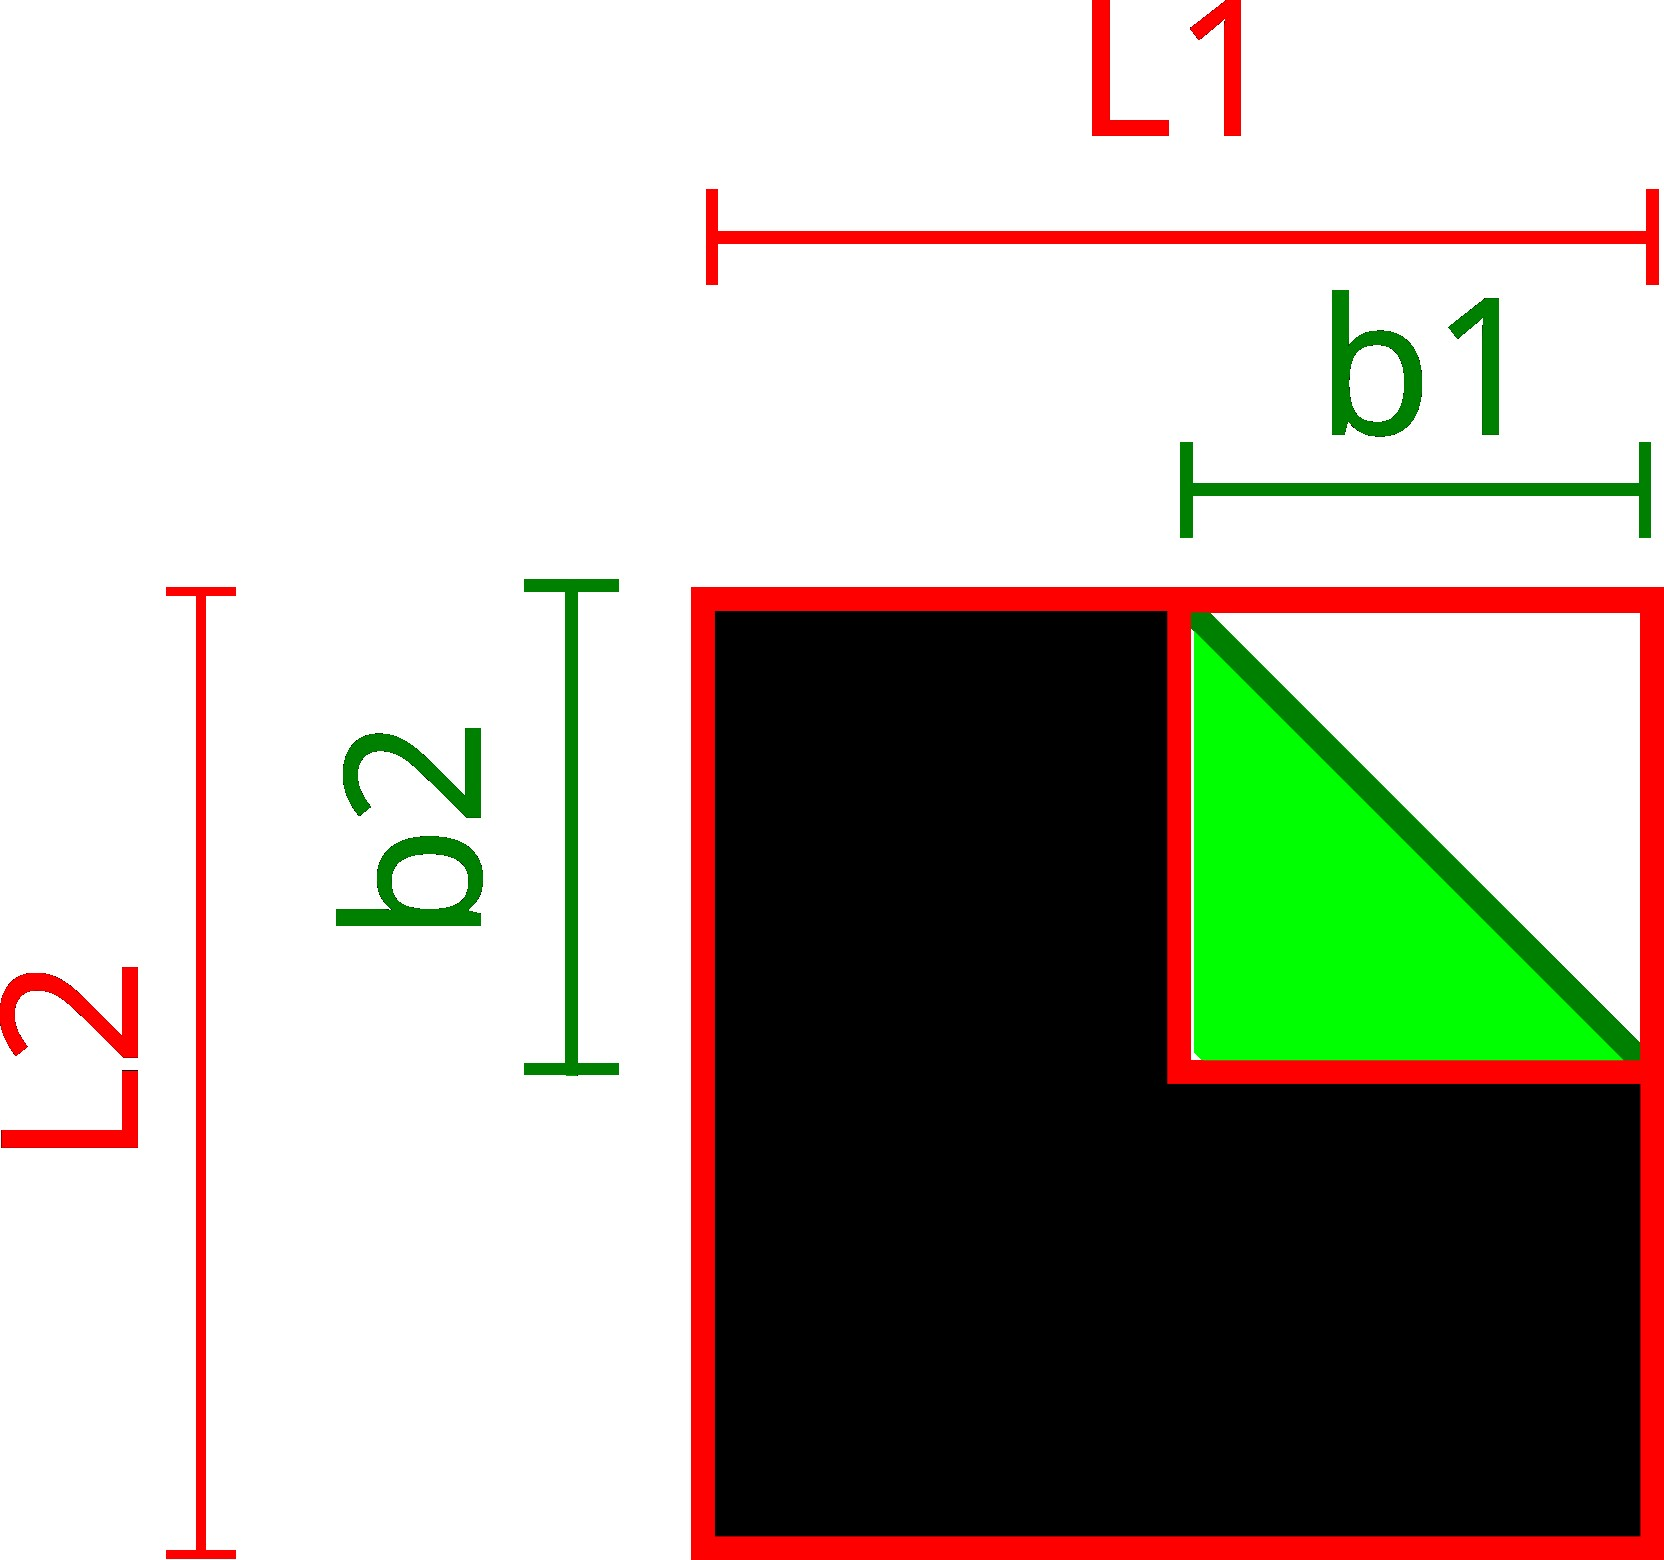
\includegraphics[width=0.6\linewidth]{figures/setback_ratio.jpg}
            \caption{Setback ratio (NTC and ASCE 7).}
            \label{fig:NTC_setback_ratio}
        \end{subfigure} & 
        \begin{subfigure}[t]{0.3\linewidth}
            \centering
            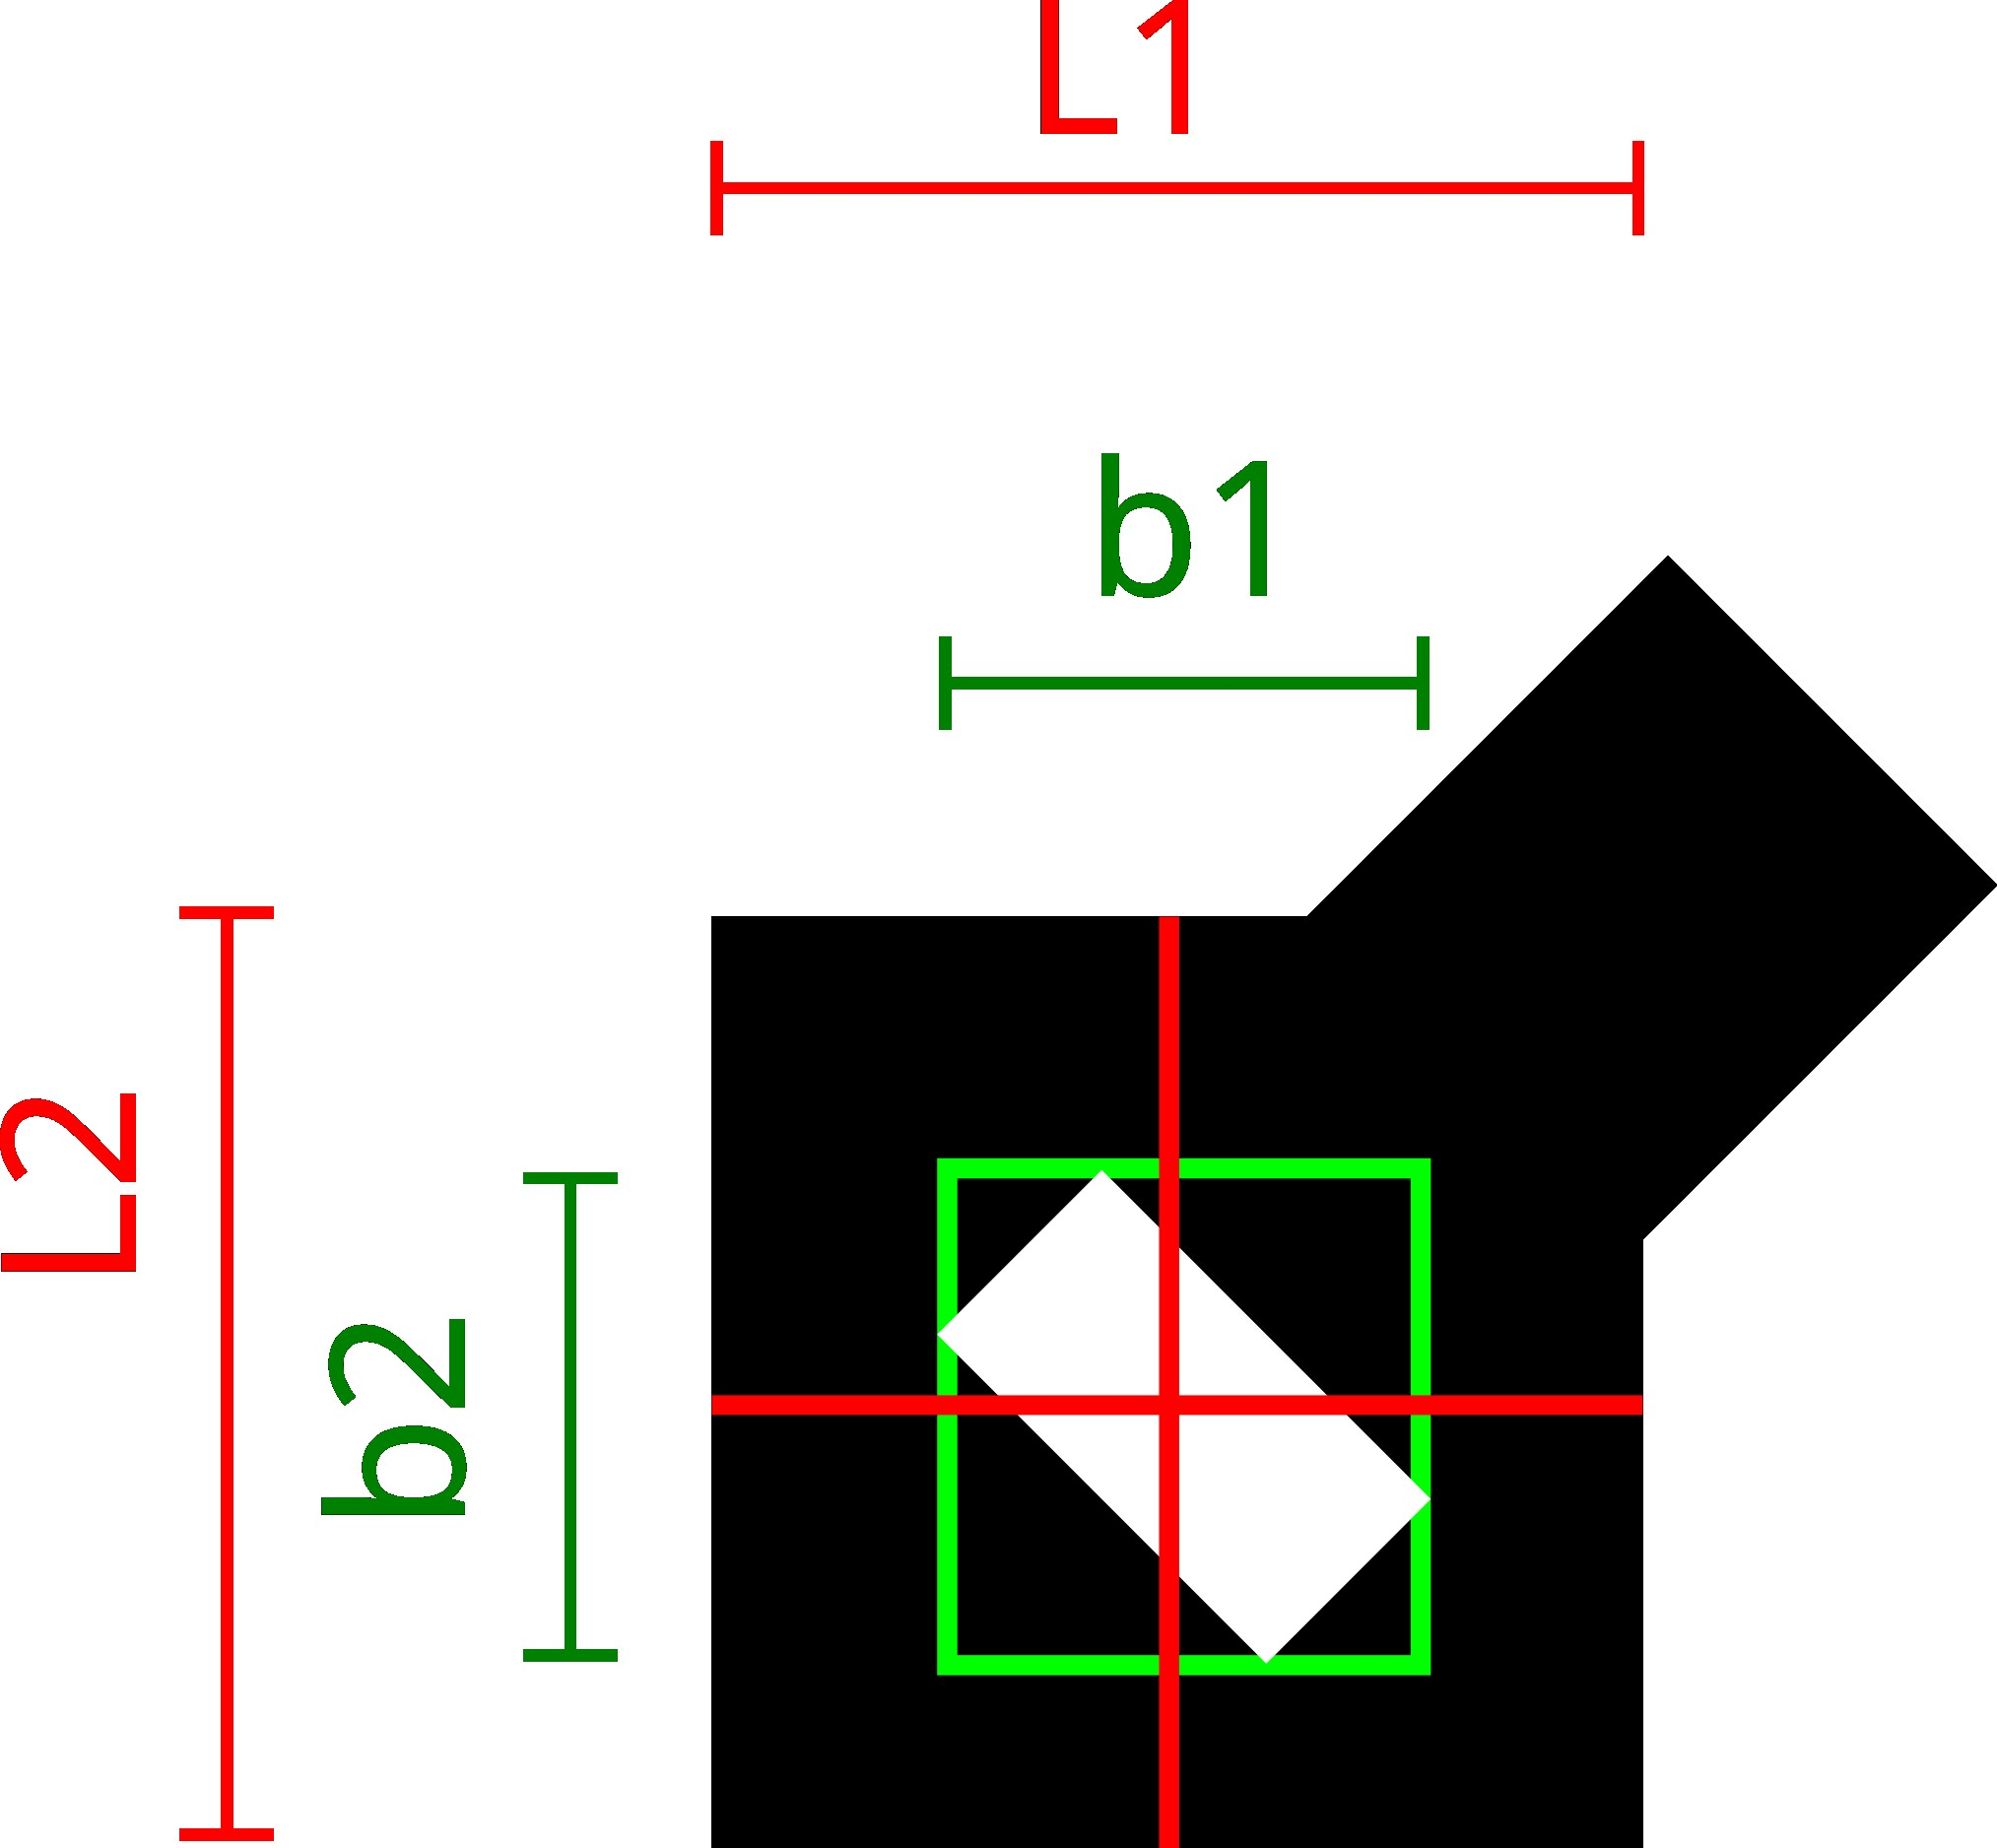
\includegraphics[width=0.6\linewidth]{figures/hole_ratio.jpg}
            \caption{Hole ratio (only NTC).}
            \label{fig:NTC_hole_ratio}
        \end{subfigure}
    \end{tabular}
    \caption{Hole and setback ratio according to the NTC code.}
    \label{fig:NTC}
\end{figure}

This study implements two geometric irregularity parameters from the Mexican building code, Norma Técnica Complementaria para el Diseño por Sismo (NTC-23) \footcite{instituto_para_la_seguridad_de_las_construcciones_norma_2023}, developed specifically for Mexico City. The first is the setback ratio, which is calculated in the same manner as in the ASCE 7 standard but allows for a less stringent threshold (fig \ref{fig:NTC_setback_ratio}). The second is the hole ratio, which is defined differently and computed according to equation \ref{eq:hole_ratio}.

\begin{equation}
    \label{eq:hole_ratio}
    \text{hole\_ratio} = \frac{h}{L}    
\end{equation}

For each identified hole, a bounding rectangle is drawn aligned with the minimum bounding box of the hole. The width of the hole is then measured ($h$).

To determine the footprint side ($L$), the direction of measurement is defined by the minimum bounding box of the hole. A measurement line is then drawn along this direction, passing through the centroid of the hole (fig \ref{fig:NTC_hole_ratio}).

The NTC-23 code sets threshold values for both parameters, as shown in table \ref{tab:MX_limits}.

\begin{table}[h]
    \centering
    \caption{Irregularity parameter limits according to the Mexican NTC-23 code.}
    \begin{tabular}{|c|c|}
        \hline
        \textbf{Parameter} & \textbf{Limit} \\
        \hline
        \textbf{Setback ratio} & $\leq 0.4$ \\
        \hline
        \textbf{Hole ratio} & $\leq 0.4$ \\
        \hline
    \end{tabular}
    \label{tab:MX_limits}
\end{table}


\renewcommand{\sectionnametext}{Footprint Shape Index (FSI)}
\renewcommand{\headingtextR}{\thesection. \sectionnametext}
\section{\sectionnametext}

The FSI is defined as a rule-based categorical descriptor of footprint-related structural regularity. It is established from three plan-based attributes commonly considered in seismic design codes: eccentricity, shape irregularity and slenderness. The FSI is not a composite numerical index and is not derived from averaging or weighting these attributes. Instead, each building is assigned to one, and only one, of four mutually exclusive categories: Regular, Eccentricity, Shape, or Slenderness.

A building is classified as \textit{regular} only if it complies with the code-prescribed thresholds for all three attributes. If at least one threshold is exceeded, the building is classified as \textit{irregular}. In such cases, the assigned FSI class identifies the governing source of irregularity. Eccentricity corresponds to non-compliance with code provisions related to plan eccentricity; Shape corresponds to non-compliance with provisions related to plan geometric irregularities, such as setbacks or holes within the footprint; and Slenderness corresponds to non-compliance with provisions related to plan slenderness.

When more than one irregularity criterion is triggered, the final classification is determined according to a hierarchical priority rule: Slenderness takes precedence over Shape, and Shape takes precedence over Eccentricity. Consequently, the FSI identifies the governing irregularity mode rather than the number of code violations. For instance, if a building does not satisfy the criteria for both slenderness and eccentricity, its FSI classification is Slenderness.

For each attribute, the reference code should be selected according to the geographical context of the study and the intended level of conservatism. In this regard, ASCE 7 and Eurocode 8 are generally more restrictive than several alternative code provisions.


\FloatBarrier

\newpage

\renewcommand{\sectionnametext}{References}
\renewcommand{\headingtextR}{\thesection. \sectionnametext}
\section{\sectionnametext}
\printbibliography[heading=none]

\end{refsection}